\documentclass{article}

% if you need to pass options to natbib, use, e.g.:
%     \PassOptionsToPackage{numbers, compress}{natbib}
% before loading neurips_2019

% ready for submission
% \usepackage{neurips_2019}

% to compile a preprint version, e.g., for submission to arXiv, add add the
% [preprint] option:
%     \usepackage[preprint]{neurips_2019}

% to compile a camera-ready version, add the [final] option, e.g.:
     \usepackage[final]{neurips_2019}

% to avoid loading the natbib package, add option nonatbib:
%     \usepackage[nonatbib]{neurips_2019}

\usepackage[utf8]{inputenc} % allow utf-8 input
\usepackage[T1]{fontenc}    % use 8-bit T1 fonts
\usepackage{hyperref}       % hyperlinks
\usepackage{url}            % simple URL typesetting
\usepackage{booktabs}       % professional-quality tables
\usepackage{amsfonts}       % blackboard math symbols
\usepackage{nicefrac}       % compact symbols for 1/2, etc.
\usepackage{microtype}      % microtypography

% My packages

\usepackage[mathscr]{euscript}
\usepackage{natbib}
\usepackage{graphicx}
\usepackage {tikz}
\usetikzlibrary {positioning}
\usepackage{amsthm}
\usepackage{amsmath}
\usepackage{amssymb}
\usepackage{dsfont}
\usepackage{hyperref}
\usepackage{stmaryrd }
\usepackage{csquotes}
\usepackage{wasysym}

\theoremstyle{plain}
\newtheorem{theorem}{Theorem}
\newtheorem{corollary}[theorem]{Corollary}
\newtheorem{lemma}[theorem]{Lemma}

\theoremstyle{definition}
\newtheorem{definition}{Definition}[section]
\newtheorem{example}{Example}[section]

\newcommand{\CI}{\mathrel{\text{\scalebox{1.07}{$\perp\mkern-10mu\perp$}}}}
\newcommand{\CII}{\mathrel{\text{\scalebox{1.07}{$\perp\mkern-10mu\perp\mkern-10mu\perp$}}}}
\newcommand{\RV}[1]{\ensuremath{\mathsf{#1}}}
\newcommand{\PA}[2]{\ensuremath{\text{Pa}_{#1}(#2)}}
\newcommand{\ND}[2]{\ensuremath{\text{ND}_{#1}(#2)}}
\newcommand{\CH}[2]{\ensuremath{\text{Ch}_{#1}(#2)}}
\newcommand{\DE}[2]{\ensuremath{\text{De}_{#1}(#2)}}
\makeatletter
\newcommand*\bigcdot{\mathpalette\bigcdot@{.5}}
\newcommand*\bigcdot@[2]{\mathbin{\vcenter{\hbox{\scalebox{#2}{$\m@th#1\bullet$}}}}}
\makeatother

\newcommand\splitter[1]{%
\begin{tikzpicture}[scale=#1]
\draw (0,-1) -- (0,0);
\draw (0,0) to [bend right] (1,1);
\draw (0,0) to [bend left] (-1,1);
\end{tikzpicture}
}

\newcommand\stopper[1]{%
\begin{tikzpicture}[scale=#1]
\draw (0,-1) -- (0,0);
\node (E) at (0,0) {$\bigcdot$};
\end{tikzpicture}
}

\DeclareMathOperator*{\argmax}{arg\,max}
\DeclareMathOperator*{\argmin}{arg\,min}
\DeclareMathOperator*{\arginf}{arg\,inf}
\DeclareMathOperator*{\argsup}{arg\,sup}

\newcommand{\cheng}[1]{ {\color{purple}[{\bf Cheng:~{#1}}]} }


\title{How to ask a causal question}

% The \author macro works with any number of authors. There are two commands
% used to separate the names and addresses of multiple authors: \And and \AND.
%
% Using \And between authors leaves it to LaTeX to determine where to break the
% lines. Using \AND forces a line break at that point. So, if LaTeX puts 3 of 4
% authors names on the first line, and the last on the second line, try using
% \AND instead of \And before the third author name.

\author{%
  David Johnston \\
  College of Engineering and Computer Science\\
  Australian National University and DATA61\\
  ACT, Australia 0200 \\
  \texttt{david.johnston1@anu.edu.au} \\
  % examples of more authors
   \And
  Cheng Soon Ong\\
  DATA61 and Australian National University\\
  % Address \\
  % \texttt{email} \\
   \And
   Robert Williamson \\
   Australian National University and DATA61\\
  % Address \\
  % \texttt{email} \\
  % \And
  % Coauthor \\
  % Affiliation \\
  % Address \\
  % \texttt{email} \\
  % \And
  % Coauthor \\
  % Affiliation \\
  % Address \\
  % \texttt{email} \\
}


\begin{document}

\maketitle

\begin{abstract}
There are multiple competing approaches to the handling of causality in statistical inference, including Causal Bayesian Networks and Potential Outcomes which differ in part in their underlying conceptions of causality. In an approach similar to Dawid, we develop the notion of a causal statistical decision problem patterned after the statistical decision theory of Wald. Our approach is motivated by a simple consideration: suppose we have a dataset, some set of available decisions and we know what state we would like the world to occupy, but we are uncertain about how our decisions affect the state of the world. We introduce the notion of \emph{consequence } that relate decisions to states of the world, and \emph{causal theories} that relate observations to consequences. These definitions are not motivated by minimal ``causal'' considerations, save the need to connect observations, decisions and consequences. We connect causal statistical decision problems to statistical decision problems via a reduction that allows results from the latter to sometimes be imported to the former. We show that Causal Bayesian Networks and Potential Outcomes both have a natural mapping to causal theories, and demonstrate a straightforward example of a causal theory that cannot be unambiguously represented by either. We argue by example that, given this more general perspective, the standard understanding of a Causal Bayesian Network is only justified under additional nontrivial assumptions. Finally, we conclude with a long list of open questions raised by this new perspective.
\end{abstract}

\section{Introduction}

% \cheng{Add a Venn diagram at the top of page 2, with all the terms in it.}

% \cheng{Do not assume your reader knows what is Causal Bayesian Networks and Potential Outcomes. You need to describe them.}

The decision theoretic approach to statistics casts statistical problems in terms of learning to output decisions that minimise a loss rather than learning true properties of a data generating distribution. Statistical decision theory plays a role of fundamental importance in modern machine learning; loss functions underpin the development of algorithms, and the analysis of losses is critical to the theoretical treatment of learning algorithms.

It is widely accepted that problems of causal inference are different to statistical problems. Causal problems are held to demand causal knowledge that is not in the vocabulary of statistical problems \citep{pearl_causality:_2009,cartwright_no_1994}. There are two leading approaches to formalising ``causal knowledge'' and posing data-driven causal problems: one based on Causal Bayesian Networks and the other on Potential Outcomes.

Causal Bayesian Networks (CBNs) posit that there are causal relationships among a set of random variables that can be encoded by a directed acyclic graph (DAG). An investigator with access to the true graph and a joint probability distribution over all the variables present in that graph can calculate a wide variety of causal effects, and partial access to these objects will enable to partial knowledge of causal effects. A causal effect in this framework is is tied to the intuitive notion of ``the result of intervening to set particular variables to particular values''.

Potential Outcomes (PO) posits a large joint distribution over observed variables $\RV{X}$, $\RV{Y}$ and partly unobserved ``potential outcome'' variables $\RV{X}_0$, $\RV{Y}_1$ and so forth. A potential outcome variable $\RV{Y}_i$ is interpreted as ``the value of $\RV{Y}$ that would be observed if the action identified by $i$ were taken''. Under some conditions, an investigator with access to a joint distribution over observed variables may be able to infer certain properties of the distribution over potential outcome variables such as $\mathbb{E}[\RV{X}_i]$.

Queries in the CBN framework may be concerned with identification of causal effects given a graph and a probability distribution (see for example \citep{tian2002general}), or with the determination of the true causal graph given just a probability distribution (see \citep{spirtes_causation_1993}). Queries in the PO framework usually concern identification of properties of the distribution of potential outcome variables known as \emph{treatment effects} given a dataset and certain assumptions about this distribution (see \citep{rubin_causal_2005,robins2010alternative}). In both cases, these queries fit the paradigm of ``determining true properties of nature'' rather than ``learning to output a decision that minimises a loss''.

The first contribution of this paper is the notion of a \emph{causal statistical decision problem} (CSDP) that proceeds from a natural extension of an ordinary statistical decision problem (SDP) introduced by \citep{wald_statistical_1950}. We suppose that, in contrast to an ordinary SDP where we have known preferences over (decision, state of nature) pairs, we know only our preferences over the \emph{outcomes} of decisions, which we represent with a utility function. Uncertainty over the consequences of decisions is represented by a \emph{causal theory} that connects observed data with \emph{consequence maps}. 

We show by a reduction that results concerning standard SDPs are also true of (at least) a subset of CSDPs.  We also show that both Causal Bayesian Networks and joint distributions over potential outcomes have a natural representation as causal theories. Together these results show, for example, that the class of Bayes decision functions is a complete class for CSDPs based on Causal Bayesian Networks provided certain conditions on the utility and size of the available set of decisions are met.

The notion of a causal theory presented here can naturally represent models cast in terms of CBNs or POs, but there are many causal theories that cannot easily be represented by either. We discuss a question motivated by this more general perspective: \emph{given a CBN with observable predictions what should be assumed when the data doesn't match these predictions?} We show that different answers to this question yield widely divergent conclusions.

One of the key strengths of our perspective is the possibility of theoretical treatment of causal learning from a viewpoint that is agnostic about the nature of ``causal knowledge''. Causal knowledge is a tricky domain from philosophy to practice, and there are many proposals for causal assumptions that do not neatly fit in either the CBN or PO camps \citep{bongers_theoretical_2016,dawid_beware_2010,bengio_meta-transfer_2019}. The theory presented here is capable of posing questions such as ``does a proposed causal learning method work?'' without first requiring commitments on the nature of causal knowledge. Substantial progress in machine learning has been the result of developing generic principles and learning techniques that are relevant to many datasets from many domains and are less reliant on the judgement of domain experts and we believe this separation of concerns is crucial to the advancement of generic techniques of causal learning.

Our approach is similar to that of \cite{dawid_decision-theoretic_2012}, but where he takes a ``bottom-up'' approach of developing a decision theoretic answer to particular causal questions, our approach is ``top-down'', proceeding from a general account of a causal problem to the particular objects needed to answer it. It also shares similarities with Causal Decision Theory developed by \cite{lewis_causal_1981}, though the connection with statistical decision theory is better understood at this point.

% There are two main assumptions used so far in pursuing generic causal inference: \emph{faithfulness} and the \emph{independence of cause and mechanism}. The assumption of faithfulness (together with the Causal Markov Condition) facilitates the exclusion of some graphical models on the basis of conditional independences found in the data \citep{spirtes_causation_1993} while the principle of independence of cause and mechanism enables the use of a number of special purpose techniques to assess the \emph{algorithmic independence} of marginal and conditional distributions which leads to preferment of some graphical models over others \citep{lemeire_replacing_2013, peters_identifiability_2012}.



% Both faithfulness and the independence of cause and mechanism are employed in learning causal Bayesian networks. While these are undoubtedly useful tools for causal reasoning, causal Bayesian networks are not ideal objects for the analysis of causal learning at a very general level:
% \begin{itemize}
%     \item There are causal models which cannot be captured by a DAG \citep{dawid_beware_2010,bongers_theoretical_2016}
%     \item There is controversy over how causal Bayesian networks should be adapted to answer counterfactual questions \citep{richardson2013single}
%     \item Under appropriate conditions, different graphs may induce the same set of interventional distributions \citep{peters_structural_2015}
%     \item A standard causal Bayesian network posits an intervention operation for every variable under consideration, while the actions to be evaluated may be much more limited. Learning such a graph appears to run afoul of Vapnik's precept: \emph{When solving a given problem, try to avoid solving a more general problem as an intermediate step} \citep{vapnik_nature_2013}
% \end{itemize}

\section{Definitions}

\cheng{One sentence describing the difference between $E$ and $\mathcal{E}$. Explicitly say that you are using caligraphic letters to mean measures, e.g. $\mathcal{G}, \mathcal{H}$ below.}

\cheng{Generally, you need to define notation (instead of expecting the reader to infer from type signatures).}

\cheng{You need to clarify the distinction between measures and probability measures.}

Given two measureable sets $(E,\mathcal{E})$ and $(F,\mathcal{F})$, a \emph{Markov kernel} $K:E\to \Delta(\mathcal{F})$ is a map where
\begin{enumerate}
    \item The map $x\mapsto K(x;B)$ is $\mathcal{E}$-measurable for every $B\in\mathcal{F}$
    \item The map $B\mapsto K(x;B)$ is a probability measure on $(F,\mathcal{F})$ for every $x\in E$
\end{enumerate}

Abusing notation somewhat, we will write the set of Markov kernels of type $E\to \Delta(\mathcal{F})$ as $\Delta(\mathcal{F})^D$.

Two Markov kernels $K:E\to \Delta(\mathcal{F})$ and $K':E\to \Delta(\mathcal{F})$ are $\mu$-almost surely equivalent given $\mu\in \Delta(\mathcal{E})$ if
\begin{align}
    \int_A K(x;B) d\mu = \int_A K'(x;B) d\mu\qquad\forall A\in \mathcal{E}, B\in\mathcal{F}
\end{align}

Given $\mu\in \Delta(\mathcal{E})$ and a sub-$\sigma$-algebra $\mathcal{D}\subset\mathcal{E}$, there is a Markov kernel $\mu_{\mathcal{D}}:E\to\Delta(\mathcal{E})$ such that for $A\in\mathcal{E}$ and $B\in \mathcal{D}$, $\int_B \mu_{\RV{X}}(y;A) d\mu(y) = \mu(A\cap B)$. $\mu_{\mathcal{D}}$ is a \emph{conditional probability distribution} with respect to $\mathcal{D}$. Given a set of random variables $\mathbf{X}=\{\RV{X}^i\}_{i\in [N]}$ with domain $(E,\mathcal{E})$, $\mu_{\mathbf{X}}$ is a conditional probability distribution with respect to the $\sigma$-algebra generated by $\mathbf{X}$: $\sigma(\cup_{i\in[N]}\sigma(\mathcal{X}^i))$.

\cheng{$D$ not defined.}

\cheng{$\Delta$ not defined.}

\subsection{Operations with Markov kernels}

For the following, assume $K$ is a Markov kernel from $E\to \Delta(\mathcal{F})$, L is a Markov kernel $F\to \Delta(\mathcal{G})$, $\mu$ is a probability measure on $(E,\mathcal{E})$ and $f$ is a nonnegative measurable function $F\to \mathbb{F}$. More details can be found in Appendix \ref{app:markov_kernels}

\cheng{$\mathbb{F}$ needs clarification.}

The notation here borrows heavily from \cite{cinlar_probability_2011} and \cite{fong_causal_2013}.

\cheng{You need to write a small tutorial about Markov kernels, otherwise reader cannot follow.}

\subsubsection{Kernel products}

\cheng{Explicitly say that $KL$ is a product of kernels $K$ and $L$. Symmetric? Distributive? Similarly for all the other products.}

$KL$ is a Markov kernel $E\to \Delta(\mathcal{G})$ such that
\begin{align}
    KL(x;B):= \int_F K(x;dy) L(y;B),\qquad x\in E, B\in \mathcal{G}
\end{align}

$\mu K$ is a probability measure on $(F,\mathcal{F})$ such that
\begin{align}
    \mu K(B)=\int_E \mu(dx) K(x;B),\qquad B\in\mathcal{F}
\end{align}

\subsubsection{Special kernels and operations}


$I_E$ is the identify kernel $E\to \Delta(\mathcal{E})$ defined by $x\mapsto \delta_x$. It has the properties $\mu I_E=\mu$, $KI_F = K$, $I_E K = K$, $I_F f=f$.
=======
\cheng{Motivate why we need these special definitions. I think the kernels are special, but operations not.}

\cheng{Also teach the reader how to say the symbols $\splitter{0.15}, \stopper{0.15}$.}



Given some measurable function $g:E\to F$, the kernel $F_g:E\to \Delta(\mathcal{F})$ is defined by $x\mapsto \delta_{g(x)}$. It is easy to check that $F_g F_g = F_g$. For $\mu\in \Delta(\mathcal{E})$, the product $\mu F_g$ is the push forward measure $g_*\mu$. 

Given $\mu\in \Delta(\mathcal{E}$, $\mu\splitter{0.15}(I_E\otimes K)$ is a distribution in $\Delta(\mathcal{E}\otimes\mathcal{F})$ given by
\begin{align}
    \mu\splitter{0.15}(I_E\otimes K)(A\times B) = \int_A K(x;B) d\mu(x)\qquad \forall A\in \mathcal{E},B\in \mathcal{F}
\end{align}


Given a set of random variables $\{\RV{X}^i\}_{i\in[N]}$ with domain $(E,\mathcal{E})$,  $\mu\splitter{0.15}(\otimes_{i\in[N]} F_{\RV{X}^i})$ is the joint distribution the set.

\cheng{Reviewers are not going to be patient enough to sit through 2 pages of definitions. You need to motivate why you need so many spaces, measures, products, etc.}


\section{Causal Statistical Decision Problems}
\begin{table}[ht]
    \centering
\begin{tabular}{ |c|c|c| } 
 \hline
  & SDPs & CSDPs \\ 
 \hline
 State of the world & $\mathscr{H}$, hypothesis class & $\mathscr{T}$, causal theory \\ 
 Observations & $\RV{X}$ & $\RV{X}$ \\ 
 Decisions & $D$ & $D$ \\
 Known preferences & $\ell$, loss & $U$, pseudo-utility \\
 Derived preferences & $\ell$, loss & $L$, causal loss\\
 \hline
\end{tabular}
    \caption{Comparison of SDPs and CSDPs}
    \label{tab:sdp_cdp_comparison}
\end{table}

We develop causal statistical decision problems (CSDPs) as an extension of statistical decision problems (SDPs) where our preferences (i.e. utility or loss) are known less directly in former case. Following \citep{toutenburg_ferguson_1967}, we consider SDPs and causal statistical decision problems CSDPs to represent normal form two person games. The games represent at the most abstract level the options and possible payoffs available to the decision maker, and this representation allows us to compare the two types of problem. In their more detailed versions,  CSDPs and SDPs differ in their representation of the state of the world and in the type of function that represents preferences. These differences are summarised in Table \ref{tab:sdp_cdp_comparison}.

\begin{definition}[Normal form two person game]
A normal form game is a triple $\langle \mathscr{S}, A, L\rangle$ where $\mathscr{S}$ and $A$ are arbitrary sets and $L:\mathscr{S}\times A\to [0,\infty)$ is a loss function.

\end{definition}
The set $\mathscr{S}$ is a set of possible states that the environment may occupy and $A$ is a set of actions the decision maker may take. The decision maker seeks an action in $A$ that minimises the loss $L$. Generally there is no action that minimises the loss for all environment states. A minimax solution is an action that minimises the worst case loss: $a^*_{mm} = \argmin_{a\in A} [\sup_{s\in \mathscr{S}} L(s,a)]$.

If the set $\mathscr{S}$ is equipped with a $\sigma$-algebra $\mathcal{S}$ and a probability measure $\xi\in \Delta(\mathcal{S})$ which we will call a ``prior'', a Bayes solution minimizes the expected risk with respect to $\xi$: $a^*_{ba} = \argmin_{a\in A} \int_{\mathcal{S}} L(s,a) \xi(ds)$.

\begin{definition}[Admissible Action]
Given a normal form two person game $\langle \mathscr{S}, A, L\rangle$, an action $a\in A$ is strictly better than $a'\in A$ iff $L(s,a)\leq L(s,a')$ for all $s\in\mathscr{S}$ and $L(s_0,a)<L(s_0,a')$ for some $s_0\in \mathscr{S}$. If only the first holds, then $a$ is as good as $a'$. An admissible action is an action $a\in A$ such that there is no action strictly better than $A$.
\end{definition}

\begin{definition}[Complete Class]
A class $C$ of decisions is a complete class if for every $a\not\in C$ there is some $a'\in C$ that is strictly better than $a$.

A class $C$ is an essentially complete class if for every $a\not\in C$ there is some $a'\in C$ that is as good as $a$.
\end{definition}

\begin{definition}[Reduction]\label{def:red_sdp_CSDP}
A normal form two person game $\alpha = \langle \mathscr{S}^\alpha, A, L^\alpha\rangle$ can be reduced to a different game sharing the same action set $\beta = \langle \mathscr{S}^\beta, A, L^\beta \rangle$ if there is a surjective function $g:\mathscr{S}^\alpha\to \mathscr{S}^\beta$ such that for every $a\in A$, $s\in \mathscr{S}^\alpha$, $L^\alpha(s,a) = L^\beta(g(s),a)$.
\end{definition}

Because CSDPs and SDPs posit states of nature of different types, they cannot represent exactly the same game. Reduction is a notion that allows us to say tht the game represented by a CSDP and an SDP are ``essentially'' the same. Reduction preserves the important properties of admissibility and completeness as shown in Appendix \ref{app:csdps}.

A statistical decision problem represents a normal form two-person game where the available actions are \emph{decision functions} that output a decision given data, the states of the environment are associated with probability measures on some measurable space and we assume a loss expressing preferences over decisions and states is known.

\begin{definition}[Statistical Decision Problem]
A statistical decision problem (SDP) is defined by a tuple $\langle (\mathscr{H},(E,\mathcal{E}), \RV{X}), (D,\mathcal{D}), \ell\rangle$. $\mathscr{H}\subset\Delta(\mathcal{E})$ is a hypothesis class representing possible states of the environment, $D$ is the set of available decisions, $\RV{X}:(E,\mathcal{E})\to (X,\mathcal{X})$ is a random variable representing the information available for the statistician to make a decision and $\ell:\mathcal{H}\times D\to [0,\infty)$ is a loss function.

Denote by $\mathscr{J}$ the set of decision kernels $X\to \Delta(\mathcal{D})$. Recall that $\mu F_{\RV{X}}(A)=\mu(\RV{X}^{-1}(A))$. For $J\in \mathscr{J}$ and $\mu\in \mathcal{H}$, the risk $R:\mathscr{J}\times\mathscr{H}\to [0,\infty)$ is defined as $R(J,\mu) = \int_D \ell(\mu,y) \mu F_{\RV{X}} J(dy)$.

Denoting by $\mathscr{J}$  the set of kernels $X\to \Delta(\mathcal{D})$, the triple $\langle \mathscr{H}, \mathscr{J}, R\rangle$ forms a two player normal form game.
\end{definition}


The loss function $\ell$ expresses preferences over (state, decision) pairs. However, it may be the case that our preferences don't naturally apply directly to such pairs. For a doctor deciding whether to prescribe a treatment to a patient, it is clear that this patient being healthy in the future is preferable to them being sick. This motivates the definition of a causal statistical decision problem, utilising a preferences defined over outcomes rather than (state, decision) pairs. In order to compute the loss associated with a decision a map from decisions to outcomes is required, which we term a \emph{consequence}.

\begin{definition}[Consequences]
Given a measurable outcome space $(F,\mathcal{F})$ and a measurable decision space $(D,\mathcal{D})$, a Markov kernel $\kappa:D \to \Delta(\mathcal{F})$ is a \emph{consequence mapping}, or just a consequence for short.
\end{definition}

\begin{definition}[Causal state]
Given a consequence $\kappa:D\to \Delta(\mathcal{F})$, a measurable observation space $(E,\mathcal{E})$ and some distribution $\mu\in \Delta(\mathcal{E})$, the pair $\tau:=(\kappa,\mu)$ is a \emph{causal state} on $D, E$ and $F$. We refer to $\kappa$ as the consequence and $\mu$ as the observed state.
\end{definition}

\begin{definition}[Causal Theory]\label{def:causal_theory}
A causal theory $\mathscr{T}$ is a set of causal states sharing the same decision, observation and outcome spaces.
\end{definition}

\cheng{You need to define the different uses of ``utility''. E.g. utility, pseudo-utility, ordinary utility, generalized utility, normal utility. Or perhaps be more careful with your usage.}

\cheng{The change from loss $\ell$ to $(U,F)$ is a surprising, so you need to explain why you need to do so.}

\cheng{The following definition is too long. Defines too many things.}

\begin{definition}[Causal Statistical Decision Problem]\label{def:CSDP}
A causal statistical decision problem (CSDP) is a tuple $\langle (\mathscr{T}, (E,\mathcal{E}) \RV{X}), (D,\mathcal{D}), (U,(F,\mathcal{F})) \rangle$. $\mathscr{T}$ is a causal theory on $D, E$ and $F$, $D$ is the decision set, $\RV{X}:(E,\mathcal{E})\to (X,\mathcal{X})$ is a random variable representing the given information and $U:\Delta(\mathcal{F}\otimes \mathcal{D})\to \mathbb{R}$ is a pseudo-utility expressing preference over joint distributions of decisions and outcomes which we assume is bounded above.

From the pseudo-utility $U$ we can define a loss $L:\mathscr{T}\times\Delta(\mathcal{D})\to [0,\infty]$ by
\begin{align}
    L((\kappa,\mu),\gamma) := \sup_{\gamma'\in\Delta(\mathcal{D})} U(\gamma'\splitter{0.15}(I_D\otimes \kappa)) - U(\gamma\splitter{0.15}(I_D\otimes \kappa))\label{eq:canonical_loss}
\end{align}
For $(\kappa,\mu)\in \mathscr{T}$ and $\gamma\in \Delta(\mathcal{D})$. This is well defined wherever $U$ is bounded above. Note that $L$ does not depend on the data generating distribution $\mu$; henceforth we will suppress this argument and write $L(\kappa,\gamma):= L((\kappa,\mu),\gamma)$.

Given a decision function $J\in\mathscr{J}$ and $(\kappa,\mu)\in \mathscr{T}$, we define the risk $R:\mathscr{J}\times \mathscr{T}\to [0,\infty)$ by $R(J,\kappa,\mu) := L(\kappa,\mu F_{\RV{X}} J)$.

The triple $\langle \mathscr{T}, \mathscr{J}, R\rangle$ is a normal form two person game.

If there exists some measurable $u:F\times D\to \mathbb{R}$ such that for all $\xi\in \Delta(\mathcal{F}\otimes\mathcal{D})$, $U(\xi)=\mathbb{E}_{\xi}[u]$ then we call $u$ an ordinary utility and by extension $U$ an ordinary pseudo-utility.

An ordinary utility induces a loss $L(\kappa,\gamma) = \mathbb{E}_{\gamma}[l^\kappa]$
where $l^\kappa:D\to [0,\infty)$ is defined by
\begin{align}
    l^\kappa(d) := \sup_{\gamma'\in \Delta(\mathcal{D})} \mathbb{E}_{\gamma'\splitter{0.08}(I_D\otimes \kappa)}[u] - \mathbb{E}_{\kappa(d;\cdot)}[u(\cdot,d)]\label{eq:induced_l}
\end{align}
\end{definition}

\cheng{Create a table that summarises the similarities and differences between the two decision problems.}

Reduction from a CSDP to an ordinary SDP is sufficient to import results from statistical decision theory such as Theorem \ref{th:complete_class}.

\cheng{Explain why complete class is important.}

\begin{theorem}[Complete class theorem (CSDP)]\label{th:complete_class}
Given an CSDP $\alpha:=\langle (\mathscr{T},E),D,\RV{X},U\rangle$ with risk $R$, if there is a reduction to an SDP $\beta:=\langle (\mathscr{H},F),D,\RV{Y},\ell \rangle$ with risk $R'$ such that $|\mathscr{H}|<\infty$ and $\inf_{J\in\mathscr{J},\mu\in\mathscr{H}} R'(J,\mu)<-\infty$, then the set of all Bayes decision functions is a complete class for $\beta$ and the set of all admissible Bayes decision functions is a minimal complete class for $\beta$.
\end{theorem}

\begin{proof}
This follows from Lemmas \ref{cor:red_comp} and \ref{lem:IB_rule}. See appendix \ref{app:csdps}.
\end{proof}

Any statistical decision problem can be reduced to a CSDP featuring a causal theory where decisions have no effect.

\cheng{Justify the choice of word ``reduce''.}


\begin{theorem}\label{th:sdp_to_CSDP}
Every SDP $\langle (\mathscr{H},E,\RV{X}),D,\ell\rangle$ can be reduced to a CSDP.
\end{theorem}
\begin{proof}
Choose a theory that matches every probability measure $\mu\in\Delta(\mathcal{E})$ with a consequence map that itself always yields $\mu$. Then construct a utility $U$ that induces an identical risk. See Appendix \ref{app:csdps}.
\end{proof}

The pseudo-utility $U$ enables Theorem \ref{th:sdp_to_CSDP}. A reduction is sometimes possible to an CSDP featuring an ordinary utility with a nontrivial theory, but whether this is always possible remains an open question.

A CSDP cannot, in general, be reduced to a statistical decision problem - for example, if we choose the utililty to be the variance of some random variable we may be able to achieve higher utility through a randomised decision than any nonrandomised decision under conditions where a regular SDP cannot have this property (see Example \ref{ex:ired_csdp} in Appendix \ref{app:csdps}). It is an open question whether this reduction is generally possible if the problem features a normal utility.

Theorem \ref{th:red_CSDP} reduces a CSDP to a SDP by associating each pair $(\mu,\kappa)$ in the causal theory with a distribution over $E\times F\times D$. This may be possible by finding a distribution on the product space for which $\mu$ is a marginal probability and $\kappa$ is a conditional distribution, but this is not necessary.

\begin{theorem}\label{th:red_CSDP}
Given a CSDP $\beta=\langle (\mathscr{T},E,\RV{X}),D,(U,F)\rangle$ where $U$ is an ordinary pseudo-utility, let $\mathscr{K}=\{\kappa|(\kappa,\mu)\in \mathscr{T}\}$ be the set of consequences. $\beta$ is reducible to a statistical decision problem on the measurable space $(E\times F\times D,\mathcal{E}\otimes \mathcal{F}\otimes \mathcal{D})$ if there is some surjective map $m:\Delta(\mathcal{F}\otimes\mathcal{D})\to \mathscr{K}$.
\end{theorem}

\begin{proof}
We construct the map $h$ based on the map $m$ and show that, given an ordinary utility $U$, it is possible to construct a loss $\ell$ such that the resulting SDP features the same risk assignments as the original CSDP. See Appendix \ref{app:csdps}.
\end{proof}

\begin{corollary}\label{cor:card_reduc}
If the cardinality of $\Delta(\mathcal{F}\otimes\mathcal{D})$ is at least as large as the cardinality of the set of Markov kernels $D\to \Delta(\mathcal{F})$ then an CSDP with an ordinary utility can always be reduced to a SDP.
\end{corollary}

\begin{proof}
This follows from Theorem \ref{th:red_CSDP} and the definition of cardinality.
\end{proof}

A major open question, then, is if $(E,\mathcal{E})$ and $(D,\mathcal{D})$ are standard measurable spaces, the conditions for Corollary \ref{cor:card_reduc} hold in general. Corollary \ref{cor:CSDP_to_sdp} shows that the reduction can be made in general if $D$ is a denumerable set.

\begin{corollary}\label{cor:CSDP_to_sdp}
A CSDP $\langle (\mathscr{T},(E,\mathcal{E}),\RV{X}),(D,\mathcal{D}),(U,(F,\mathcal{F}))\rangle$ where $D$ is a denumerable set and $U$ is an ordinary pseudo-utility can be reduced to a statistical decision problem.
\end{corollary}

\begin{proof}
Take some probability measure $\pi\in \Delta(\mathcal{D})$ such that $\pi(\{y\})>0$ for all $y\in D$. Such a $\pi$ exists by the denumerability of $\mathcal{D}$. The map $m:\Delta(\mathcal{F}\otimes\mathcal{D})\to \mathscr{K}$ given by $m(\xi)(y;A) := \frac{\xi(A\times\{y\})}{\pi(\{y\})}$ is surjective. The result follows from Theorem \ref{th:red_CSDP}.
\end{proof}

This reduction is not particularly practically useful, but it is sufficient to lift results such as Theorem \ref{th:complete_class} from the theory of statistical decision functions.

\section{Causal Bayesian Networks}

A causal Bayesian network is an example of an identifiable causal theory. Given a measurable space $(X,\mathcal{X})$ where $X=\times_{i\in [N]} X^i$, a decision space $D = \times_{i\in [N]} X^i\cup\{*\}$ and a causal graph $\mathcal{G}$ over nodes $\mathbf{V}=\{V^i|i\in [N]\}$, the graph $\mathcal{G}$ maps each probability distribution $\mu\in \Delta(\mathcal{X})$ to a unique consequence $D\to \Delta(\mathcal{X})$.

The CBN convention is to call the elements of the decision space $D$ ``interventions'' and denote then with $P(\cdot|do(\cdot\cdot))$ notation. In the first definition below, we instead denote interventions with indices on the probability distribution, and introduce the special $*$ object to denote a passive intervention.

\begin{definition}[Causal Bayesian Network]\label{def:CBN}
The definition here follows \cite{pearl_causality:_2009}.

Consider a directed acyclic graph $\mathcal{G}$ with nodes $\mathbf{X}=\{\RV{X}^i|i\in [N]\}$, a measurable space $(E,\mathcal{E})$ and a set of random variables $\RV{X}^i:E\to X^i$ and let $X=\times_{i\in[N]} X^i$. For each $x\in \times_{i\in [N]} X^i\cup \{*\}$ suppose we have an \emph{interventional distribution} $P^{x}\in \Delta(\mathcal{E})$, and let the set of all such distributions be denoted $\mathbf{P}^{X\cup\{*\}}$. Let $P^*$ be the passive distribution given by the intervention $x = (*,...,*)$.

Given any $x\in X\cup\{*\}$ let $S(x)\subset[N]$ be the set of all indices $i$ such that $x^i\neq *$. The graph $\mathcal{G}$ is a causal Bayesian network compatible with $\mathbf{P}^{X\cup\{*\}}$ iff for all $x\in X$ and $S(x)\subset [N]$:
\begin{enumerate}
    \item $P^{x}_{\RV{X}}$ is compatible with $\mathcal{G}$ for all $x\in \cup_{i\in [N]} X^i\cup \{*\}$
    \item $P^x_{\RV{X}}(\RV{X}^{S(x)})=\delta_{x^{S(x)}}(\RV{X}^{S(x)})$
    \item For $i\in S^C$, $P^x_{\RV{X}}(\RV{X}^i|\PA{\mathcal{G}}{\RV{X}^i})=P^*_\RV{X}(\RV{X}^i|\PA{\mathcal{G}}{\RV{X}^i})$, $P^x$-almost surely
\end{enumerate}
\end{definition}

The above three conditions are sufficient that, given some graph $\mathcal{G}$ and $P^*_{\RV{X}}\in \Delta(\mathcal{X})$, one obtains a unique set of interventional distributions $\mathbf{P}_{\mathcal{G}}^{X\cup\{*\}}$ (this follows from the truncated factorisation property given by \cite{pearl_causality:_2009}). Identifying the decision set $D$ with $\times_{i\in [N]} X^i\cup\{*\}$, note that the map $\kappa^P_\mathcal{G}:D\to \Delta(\mathcal{X})$ given by $d\mapsto P^d_{\mathcal{G}}$ looks like a consequence map, which in fact it is (as established by Theorem \ref{th:cbn_MK}). The set of pairs $\{(P^*_{\RV{X}}, \kappa^P_\mathcal{G})|P^*_{\RV{X}}\in \Delta(\mathcal{X})\}$ is then a causal theory $\mathscr{T}_\mathcal{G}$.

\begin{theorem}\label{th:cbn_MK}
Given a graph $\mathcal{G}$, a measurable set $(E,\mathcal{E})$ and a decision set $D=\times_{i\in [N]} X^i\cup\{*\}$, let $P^x\in \Delta(\mathcal{E})$ be an interventional distribution compatible with $\mathcal{G}$ as defined in Definition \ref{def:CBN}. 

Then the map $\kappa_{\mathcal{G}}:D\to \Delta(\mathcal{X})$ given by $x\mapsto P^x$ is a Markov kernel.
\end{theorem}

The proof is given in Appendix \ref{app:cbn_ct}.

\subsection{Extending the theory induced by a CBN}

The causal theory associated with a given graph $\mathcal{G}$ is in general incomplete in that it does not associate a consequence with some distributions on $\Delta(\mathcal{X})$. In particular, if certain conditional independences are implied by $\mathcal{G}$, then probability distributions for which these conditional independences do not hold do not appear in the associated causal theory - only \emph{compatible} distributions are represented. This follows from condition 1 of Definition \ref{def:CBN}. While a theory doesn't have to feature a causal state for every possible distribution, it usually isn't reasonable to assume \emph{a priori} that certain conditional independences hold. In this case, it is necessary to extend the causal theory associated with $\mathcal{G}$ to cover distributions that are incompatible with $\mathcal{G}$.

The choice of how to extend the theory can be important. For discrete and jointly Gaussian distributions, conditional independences are associated with lower dimensional subspaces of the set of distributions\cite{meek_strong_1995}. Given causal theory $\mathscr{T}\subset$ and a $\sigma$-algebra $\mathcal{T}$, if we have a prior $\xi\in \Delta(\mathscr{H}\times \mathscr{K})$ such that the marginal $P^\xi(A)$ for $A\in \Delta(\mathscr{H})$ admits a density $P^\xi(A) = \int_A p^\xi(x)dx$ then this prior will assign 0 weight to any subset of $\mathscr{T}$ for which some conditional independence holds, and so for any $\mathcal{G}$ which is not fully connected the Bayes risk of any decision function $J$ is determined entirely by the extension of $\mathscr{T}$ to the set of distributions incompatible with $\mathcal{G}$.

An example follows. Suppose we have the following graph $\mathcal{G}$:

\begin{figure}
    \centering
     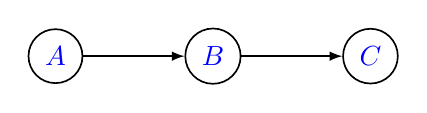
\begin{tikzpicture}[-latex,auto ,node distance =1 cm and 2cm ,on grid ,
    semithick ,
    vb/.style ={ circle ,top color =white , 
    draw , text=blue , minimum width =0.6 cm},
    kernel/.style={rectangle,draw}
    ]

    \node[vb] (A) {$A$};
    \node[vb] (B) [right = of A] {$B$};
    \node[vb] (C) [right = of B] {$C$};
    \draw (A) -- (B);
    \draw (B) -- (C);
    \end{tikzpicture}
    \caption{Simple causal Bayesian network $\mathcal{G}$}
    \label{fig:simple_cbn}
\end{figure}

Associated with this graph is the sample space $(E,\mathcal{E})=(\{0,1\}^3,\mathscr{P}(\{0,1\}^3)$ where $\mathscr{P}$ denotes the power set, and random variables $\RV{A},\RV{B}$ and $\RV{C}$ taking values in $\{0,1\}$. The set of possible distributions $\Delta(\mathcal{E})$ can be identified with the probability simplex in $\mathbb{R}^8$. For simplicity, suppose that only $A$ can be intervened on; that is, the decision space $D=A\cup\{*\}$ with the decision $\RV{D}_A=x$ for $x\in A$ having the usual interpretation as a hard intervention on $A$. We could alternatively assign infinite costs to interventions on $B$ and $C$, but this adds unnecessary complexity.

$\mathcal{G}$ implies $\RV{A}\CI \RV{C} | \RV{B}$. We have a theory $\mathscr{T}_{\mathcal{G}}$ associated with the graph $\mathcal{G}$ containing the state
\begin{align}
    (\nu,x\mapsto P^\nu(\RV{B}|\RV{A}=x) ) \label{eq:ocbn}
\end{align}
for every compatible $\nu$ . 

Consider two options for extending this to distributions $\nu$ incompatible with $\mathcal{G}$:
\begin{itemize}
    \item $\mathscr{T}_{\mathcal{G}}'$ assigns the causal states given by the union over all DAGs on the set of nodes $\{A, B, C\}$
    \item $\mathscr{T}_{\mathcal{G}}^\square$ assigns the causal states given by the union over all supergraphs of $\mathcal{G}$ on $\{A, B, C\}$
    \item $\mathscr{T}_{\mathcal{G}}^\circ$ assigns the causal states given by $\mathcal{G}$ and ignores the inconsistency of $\nu$
\end{itemize}

In the first theory, for every DAG featuring $A\to B$ there is a DAG featuring $B\to A$; in addition, there are a number of DAGs with no arrow between $A$ and $B$. Therefore any prior $\xi$ that admits a density over $\Delta(\mathcal{E})$ and assigns equal weight to each causal state in $\mathcal{T}$ featuring the same distribution will generate a posterior that assigns a weight of more than 0.5 to the possibility that the marginal distribution of $\RV{B}$ is independent of whatever decision $\RV{D}_A$ is chosen. This remains true even if the observed data consist of a very large number of IID observations distributed according to some $\pi$ for which it is indeed holds that $\RV{A} \CI_\pi \RV{C} | \RV{B}$.

The second theory, on the other hand, yields a set consequences that are ``close'' to the consequence given by the original graph $\mathcal{G}$ provided the distribution $\mu$ is sufficiently ``close'' to a distribution $\nu$ for which $\RV{A} \CI_\nu \RV{C} | \RV{B}$. Note that, marginalising over $\RV{A}$ and $\RV{C}$ and ignoring the passive action, the theory $\mathscr{T}^\square_{\mathcal{G}}$ associates two consequences with every incompatible $\mu$:
\begin{align}
    &(\mu,x\mapsto P^\mu(\RV{B}|\RV{A}=x) )\label{eq:cbn_s1}\\
    &(\mu,x \mapsto \sum_c P^\mu(\RV{B}|\RV{A}=x,\RV{C}=c)P^\mu(\RV{C}=c)) \label{eq:cbn_s2}
\end{align}

Note that \ref{eq:cbn_s1} matches the pattern for states in the original graph \ref{eq:ocbn}. Define the consequences $\kappa^\circ := x\mapsto P^\mu(\RV{B}|\RV{A}=x)$ and $\kappa^\square:= x \mapsto \sum_c P^\mu(\RV{B}|\RV{A}=x,\RV{C}=c)P^\mu(\RV{C}=c))$, leaving the $\mu$-dependence implicit.

Consider some $\mu$ for which $\RV{A} \CI_\mu \RV{C} | \RV{B}$ holds approximately. That is, for some $\epsilon>0$
\begin{align}
    \left|\sum_c P^\mu(\RV{B}|\RV{A}=x,\RV{C}=c)P^\mu(\RV{C}=c)-P^\mu(B|A=x)\right| &< \epsilon \label{eq:app_ci}
\end{align}

Suppose that we have some loss such that $L(\rho)= \mathbb{E}_\rho[\RV{B}] + k$. Noting that $\mathscr{T}^\circ_\mathcal{G}$ and $\mathscr{T}^\square_\mathcal{G}$ agree on $\kappa^\circ$, we can bound the disagreement between the two theories with
\begin{align}
    |R(J,\kappa^\square,\mu) - R(J,\kappa^\circ,\mu)| &=  \left|\mathbb{E}_{\mu J \kappa^\square} [\RV{B}] - \mathbb{E}_{\mu J \kappa^\circ} [\RV{B}]\right|\\
        &\leq \max_x \left|\sum_c P^\mu(\RV{B}|\RV{A}=x,\RV{C}=c)P^\mu(\RV{C}=c)-P^\mu(B|A=x) \right|\\
        &< \epsilon
\end{align}

The stipulation that the prior $\xi$ was such that the marginal distribution over $\Delta(\mathcal{E})$ admitted a density may be controversial. It is consistent with the notion that ``there are no true parametric zeros'' endorsed by many statisticians (for example  \cite{gelman_bayesian_2010,meehl_theory-testing_1967,berkson_difficulties_1938}). Furthermore, if conditional independences rarely hold precisely, then learners based on the theory $\mathscr{T}_{\mathcal{G}}'$ may usually converge to a state of skepticism even given a prior that assigns nonzero weight to the set of compatible probability distributions because the data are usually drawn from a distribution from which this independence does not hold.

\textbf{TODO (maybe)} A useful property to consider of causal theories is whether determining the data generating distribution $\mu$ is ``close'' to $\mu_0$ implies that the risk is ``close'' to $R(J,\mu_0,\kappa_0)$ for all $(\mu_0,\kappa_0)$ in $\mathscr{T}$. One has to choose a reasonable notion of closeness. There are possible results in the spirit of the example above for Bayesian networks.

\section{Potential Outcomes}

\textbf{Todo: } This story could be made stronger starting from the proposition that using PO or anything else, you still need to rate the desirability of available decisisons somehow.

Potential outcomes provide an alternative means to discuss causal effects. The standard setup posits a joint distribution between observed data $\RV{X}$, a treatment $\RV{Z}$ taking values in $[N]$ and several ``potential outcomes'' $\RV{X}_i$, $i\in [N]\setminus\{0\}$. At a minimum, the consistency condition is usually asserted (\cite{richardson2013single}): $\RV{Z}=i$ implies $\RV{X}_i=\RV{X}$. 

We modify this setup somewhat in order to analyse it in terms of a causal theory. We believe these choices are reasonable, but there is an element of interpretation involved here. For clarity every variable gets a subscript and $\RV{X}_{ob}$, $\RV{Z}_{ob}$ are random variables representing outcomes and treatments in the observed data. $\RV{X}_i, \RV{Z}_i$, $i\geq 0$ are random variables representing outcomes and treatments in consequence of choosing a decision $\RV{D}=i$ deterministically. Note that we do not necessarily have a ``passive decision'' as we did with CBNs. Finally, we work with a slightly weaker ``almost certain consistency'':

\begin{align}
    P(\RV{X}_i,\RV{X}_{ob}|\RV{Z}_{ob}=i,\RV{Z}_i=i)=\mathds{1}_{\RV{X}_{ob}=\RV{X}_i} \qquad\text{ with probabiliy 1}\label{eq:consistency}
\end{align}

Conditioning on $\RV{Z}_i=i$ is redundant under the usual assumption that $P(\RV{Z}_i) = \delta_i(\RV{Z}_i)$.

While there appears to be a natural identification of ``potential outcomes'' with consequences, observed data with observed state and treatments with decisions in a causal theory, it is usually not possible to represent a joint distribution obeying Condition \ref{eq:consistency} with a causal theory. Take the spaces $D,X,Z=\{0,1\}$ and suppose we have a causal theory $\mathscr{T}$ consisting of pairs $(\kappa,\mu)$ where $\mu\in\Delta(\mathcal{X}\otimes\mathcal{Z})$ and $\kappa$ is a Markov kernel from $D\to \Delta(\mathcal{X}\otimes\mathcal{Z})$. To construct a joint distribution between $\RV{X}_{ob}$ and $\RV{X}_i$ for $i\in \{0,1\}$ we take some deterministic decision function $J_i:X\times Z\to \Delta(\mathcal{D})$ where $J_i:(x,z;d)\mapsto \delta_i(d)$. For $A,C\in \Delta(\mathcal{X}\otimes\mathcal{Z})$, $B\in \Delta(\mathcal{D})$ we compose the objects as 
\begin{align}
    \xi(A\times B\times C) =  \int_B \int_A  \kappa(y; C) \delta_i(dy) \mu(dx\times dz)
\end{align}

For $\alpha\in\{ob,0,1\}$ take random variables $\RV{X}_\alpha:(X\times Z)^2\times D\to X$, $\RV{Z}_\alpha:(X\times Z)^2\times D\to X$ and $\RV{D}:(X\times Z)^2\times D\to D$ defined by projections $\RV{X}_\alpha:((x_{ob},z_{ob}),(x_i,z_i),d)\mapsto x_\alpha$, $\RV{Z}_\alpha$ similarly and $\RV{D}:((x_{ob},z_{ob}),(x_i,z_i),d)\mapsto d$. It is then straightforward to show that $(x,z,d))\mapsto \kappa(d; C)$ is a version of the conditional probability $P^\xi(\RV{X}_i|\RV{D},\RV{X}_{ob},\RV{Z}_{ob})$, which implies 
\begin{align}
    \RV{X}_i&\CI_\xi \RV{X}_{ob}|\RV{D}, \RV{Z}_{ob}
\end{align}
For any choice of $J_i,\mu,\kappa$. Noting that $J_i$ is deterministic, we also have
\begin{align}
    \RV{X}_i&\CI_\xi \RV{X}_{ob}|\RV{Z}_{ob} \label{eq:decision_d_sep}
\end{align}
Conditions \ref{eq:consistency} and \ref{eq:decision_d_sep} can hold simultaneously only if $\RV{X}_i$ and $\RV{X}_{ob}$ are deterministic conditional on $\RV{Z}_{ob}$. This is usually not the case.

In order to facilitate nontrival joint distributions between obsevations and potential outcomes, we introduce a \emph{generalised consequence}:

\begin{definition}[Generalised consequence]
Given a measurable consequence space $(F,\mathcal{F})$, a sample space $(E,\mathcal{E})$ and a measurable decision set $(D,\mathcal{D})$, a Markov kernel $\kappa:D\times E \to \Delta(\mathcal{F})$ is a generalised consequence.
\end{definition}

\begin{definition}[Generalised causal theory]
A generalised causal theory is the analogue of a causal theory with the consequence replaced by a generalised consequence.
\end{definition}

Given $D,X,Z$ as before, we provide an explicit construction respecting \ref{eq:consistency}. Here, for convenience, we identify $E=F=X\times Z$. For $x\in X$, $z\in Z$, $d\in D$ and $G\in \mathcal{X}$, $H\in \mathcal{Z}$ consider the kernel

\begin{align}
    \iota: (d,x,z;G\times H) \mapsto \delta_d(H)(\delta_z(H) \delta_x(G) + (1-\delta_z(H)) \iota'(d,x,z;G))
\end{align}

Where $\iota'$ is an arbitrary Markov kernel $D\times X\times Z\to \Delta(\mathcal{X}\otimes\mathcal{Z})$. It is straightforward to check that $\iota$ is a Markov kernel. Take the Consider the distribution given by
\begin{align}
    \zeta (A\times B\times C) =  \int_B \int_A  \iota(y,x,z; C) \delta_i(dy) \mu(dx\times dz)
\end{align}
And random variables $\RV{X}_i$, $\RV{Z}_i$ and $\RV{D}$ as before. Then
\begin{align}
    P^\zeta(\RV{X}_i=j,\RV{X}_{ob}=k|\RV{Z}_{ob}=i)P^\zeta(\RV{Z}_{ob}=i) &= \sum_{m,n} \iota(n,k,i;\{j,m\}) \delta_i(\{n\}) \mu(k,i)\\
     &= \sum_{m,n} \delta_n(m)[\delta_i(m) \delta_k(j) + (1-\delta_i(m))\iota'(n,k,i;\{j,m\})]\delta_i(\{n\}) \mu(k,i)\\
     &= \delta_k(j) \mu(k,i)
\end{align}

Which implies \ref{eq:consistency}.

\subsection{Causal Theories and Generalised Causal Theories}


A generalised causal decision problem is a causal decision problem featuring a generalised causal theory and a loss $L:\Delta(\mathcal{E}\otimes\mathcal{D}\otimes\mathcal{F})\to[0,\infty]$. There is a straightforward identification of causal theories with generalised causal theories, befitting the name. We might also ask when the extra structure of a generalised causal decision problem is needed.

Given an ordinary consequence $\kappa:D\to \Delta(\mathcal{F})$, we can trivially construct a generalised consequence $\iota:(d,e;A)\mapsto \kappa(d;A)$. In addition, given a loss $L:\Delta(\mathcal{D}\otimes\mathcal{F})\to[0,\infty]$ we can construct $L':\Delta(\mathcal{E}\otimes \mathcal{D}\otimes\mathcal{F})\to[0,\infty]$ by $L':\mu\mapsto L(\mu(E\times \cdot \times \cdot \cdot))$.

Given a generalised consequence $\iota:D\times E\to \Delta(\mathcal{F})$ and a hypothesis class $\mathscr{H}\subset\Delta(\mathcal{F})$, we can construct a causal theory $\mathscr{T}_{\iota,\mathscr{H}} = \{(d\mapsto (\mu\otimes \delta_d)\iota,\mu)|\mu\in \mathscr{H}\}$. This causal theory ``forgets'' the joint structure induced by $\iota$. For many practical problems, this extra structure is unnecessary.

Suppose $E=F=\{0,1\}^\mathbb{N}$ and $\RV{X}_{<N}=\otimes_{i\in [N-1]} \underline{\RV{X}_i}$ represents the ``past'' data while $\RV{X}_{\geq N}=\otimes_{i\geq N} \underline{\RV{X}_i}$ represents ``future'' data. Then, given some loss $L':\Delta(\mathcal{E}\otimes \mathcal{D}\otimes\mathcal{F})\to[0,\infty]$ that depends only on the distribution of the future data $\RV{X}_{\geq N}$ and $\RV{D}$, and if 

If a loss function over $\Delta(\mathcal{D}\otimes\mathcal{F})$ is sufficient to describe our preferences then any counterfactual decision problem can be posed as a regular causal decision problem.

\subsubsection{Acyclic Structural Equation Models}

An acyclic structural equation model can be understood as a special case of a generalised consequence. Recall that an acyclic structural equation model is a set of equations $M=\{X^i = f(X^{<i},\epsilon^i)|i\in[N]\}$ along with an intervention operation that replaces the right hand side of an arbitrary subset of equations with an arbitrary set of (allowable) chosen values. Identify the sample space $E=\mathbb{R}^N$ as the space from which the noises $\epsilon=(\epsilon^0,..,\epsilon^N)$ are drawn the decision set $D$ with the set of allowable interventions (including non-interventions) and $F$ as the space in which $X=(X^0,...,X^N)$ lives. Then $M$ is a function from $D\times E\to F$. We can associate the function $M$ with the kernel $\kappa_M: D\times E\to \Delta(\mathcal{F})$ by $\iota_M:(d,e;A)\mapsto \delta_{M(d,e)}(A)$.

An acyclic SEM $M$ with independent noises can be associated with a causal theory. Take a hypothesis class $\mathscr{H}\subset\Delta(\mathcal{E})$ such that for every $\mu\in\mathscr{H}$ the noises are jointly independent. Then we can associate such an SEM with the causal theory
\begin{align}
    \mathscr{T} = \{(\iota_M,(\mu\otimes \delta_*)\iota_M )|\mu\in\mathscr{H}\}
\end{align}
Where $\delta_*$ is the distribution over $D$ that assigns weight 1 to the non-intervention $*$.
%!TEX root = main.tex

\section{Potential outcomes models}\label{sec:counterfactuals}

We follow \cite{rubin_causal_2005} for the definition of a potential outcomes model, noting any points of divergence. 

Notationally, we will refer to the symbol $\RV{W}_i$ as the $i$-th treatment assignment ($i\in \{0,..,n\}$), $\RV{Y}_i(0)$ $\RV{Y}_i(1)$ as the $i$-th potential outcomes, $\RV{Y}_i$ as the $i$-th obseved outcome and $\RV{X}_i$ as the $i$-th ``vector of background facts''. $\RV{W}$ refers to the bundle of all $\RV{W}_i$s and similarly for other symbols. Following the convention set out in our introduction, we consider these symbols to represent random variables and to label strings in our string diagram. Suppose the vector $[\RV{Y}_0,...,\RV{Y}_n]$ takes values in $Y$ and similarly for other symbols.

Given an underlying state space $\Theta$, a potential outcomes model $\mathscr{O}$ consists of a set of Markov kernels $\langle \mathbf{P}, \mathbf{W}, \mathbf{Y} \rangle$ and a canonical composition that yields a statistical experiment $\mathbf{H}:\Theta\to \Delta(\mathcal{X}\otimes\mathcal{Y}\otimes \mathcal{W})$. 

The kernels are
\begin{itemize}
\item A ``model on the science'', $\mathbf{P}:\Theta \to \Delta(\mathcal{X}\otimes\mathcal{Y}\otimes\mathcal{Y})$ (In Rubin's notation, $mathbf{P}$ is $\prod_i f(\RV{X}_i,\RV{Y}_i(0),\RV{Y}_i(1)|\theta)$)
\item An ``assignment mechanism'', $\mathbf{W}:\Theta\times X\times Y^2 \to \Delta(\{0,1\}^n)$ (in Rubin's notation, $\mathbf{W}$ is $Pr(\RV{W}|X,Y(1),Y(0))$)
\item An ``observation model'', $\mathbf{Y}:\{0,1\}^n\times Y^2\to \Delta(\mathcal{Y})$, defined explicitly as $\mathbf{Y}:(\mathbf{y}^0,\mathbf{y}^1,\mathbf{w})\mapsto (1-\mathbf{w}) \odot \delta_{\mathbf{y}^0} + \mathbf{w} \odot \delta_{\mathbf{y}^0}$ where $\odot$ is the elementwise product
\end{itemize}

We differ from Rubin by defining $\mathbf{Y}$ as a Markov kernel rather than a function. This approach means that we can at best assert $W_i=w\implies \RV{Y}_i=\RV{Y}_i(w)$ \emph{almost surely} in some probability space, as a Markov kernel cannot guarantee exact equality. We also differ from Rubin by including $\Theta$ in the domain of $\mathbf{W}$ as in our framework leaving this dependence out is equivalent to assuming that the treatment assignment mechanism is known \emph{a priori} (as a result, our state $\Theta$ is larger than Rubin's).

We then define the \emph{canonical experiment} $\mathbf{H}^{\mathscr{O}}$ by

\begin{align}
\mathbf{H}^{\mathscr{O}}:=
\begin{tikzpicture}
	\path (0,0) coordinate (A)
	++ (0.5,0) coordinate (copy0)
	++ (1,0) coordinate (cent0)
	+(0,0.5) node[kernel] (HPO) {$\mathbf{P}$}
	+(0.5,0.4) coordinate (copy1)
	++ (1.3,0) coordinate (cent1)
	+(0,-0.5) node[kernel] (HW) {$\mathbf{W}$}
	++(1,0) coordinate (cent2)
	+ (0,0) node[kernel] (HY) {$\mathbf{Y}$}
	++(1,0) coordinate (cent3)
	+(0,0.65) node (X) {$X$}
	+(0,0) node (Y) {$Y$}
	+(0,-0.5) node (W) {$W$};
	\draw (A) -- (copy0);
	\draw (copy0) to [bend left=20] (HPO);
	\draw (copy0) to [bend right=20] ($(HW.west)+(0,-0.1)$);
	\draw ($(HPO.east)+(0,-0.1)$) -- (copy1);
	\draw (copy1) edge[out=0,in=180] (HW);
	\draw ($(HPO.east)+(0,0.15)$) -- (X) (HY) -- (Y) (HW) -- (W);
	\draw (copy1) edge[out=0,in=180] ($(HY.west)+(0,0.1)$);
	\draw ($(HW.east)+(0,0.1)$) to [bend left = 20] ($(HY.west)+(0,-0.1)$);
\end{tikzpicture}
\end{align}

The internal wire from $\mathbf{P}$ to $\mathbf{Y}$ and $\mathbf{W}$ carries the bundle of potential outcomes $\RV{Y}(0)\underline{\otimes}\RV{Y}(1)$. This is consistent with Rubin, though the notation is substantially different.

% Where we have labeled the wires ``carrying'' $\RV{Y}(0)$ and $\RV{Y}(1)$ for clarity. Addtionally, we could draw an alternative diagram where each wire was copied $n$ times to reflect the unit level variables. We can define an extended probability space $H^*$ on which potential outcomes are also random variables:

% \begin{align}
% H^*:=\begin{tikzpicture}
% \path (0,0) coordinate (A)
% ++ (0.8,0) node[kernel] (HPO) {$H_{PO}$}
% ++ (0.8,0) coordinate (copy00)
% + (0,0.15) coordinate (copy01)
% + (0,-0.15) coordinate (copy02)
% ++(0.8,0) node[kernel] (HW) {$H_W$}
% +(0.2,-0.6) node (Y0) {}
% +(0.2,-1.2) node (Y1) {}
% ++(0.8,0) coordinate (copy1)
% ++(0.8,0) node[kernel] (HY) {$H_Y$}
% ++(0.8,0) node (Y) {$\RV{Y}$}
% +(0,0.5) node (W) {$\RV{W}$}
% +(0,1) node (X) {$\RV{X}$}
% +(0,-0.6) node (Y0l) {$\RV{Y}(0)$}
% +(0,-1.2) node (Y1l) {$\RV{Y}(1)$};
% \draw (A) -- (HPO) -- (HW) -- (HY) -- (Y);
% \draw ($(HPO.east)+(0,0.15)$) -- ($(HW.west)+(0,0.15)$);
% \draw ($(HPO.east)+(0,-0.15)$) -- ($(HW.west)+(0,-0.15)$);
% \draw (copy01) to [bend left] (X);
% \draw (copy00) to [bend right] (Y0) to [bend right] ($(HY.west)+(0,-0.1)$);
% \draw (copy02) to [bend right] (Y1.west) -- (Y1.east) to [bend right] ($(HY.west)+(0,-0.15)$);
% \draw (copy1) to [bend left] (W);
% \draw (Y0) -- (Y0l);
% \draw (Y1) -- (Y1l);
% \end{tikzpicture}
% \end{align}

% Following this example, we will define a potential outcomes model with $m$ potential outcomes as three Markov kernels $\langle \mathbf{P}, \mathbf{W}, \mathbf{Y} \rangle$ where $\mathbf{P}:\Theta\to \Delta(\mathcal{X}\otimes\mathcal{Y}^m)$, $\mathbf{W}:\Theta\times X\times Y^m\to \Delta([m]^n)$ and $\mathbf{Y}:[m]^n\times Y^m\to \Delta(\mathcal{Y})$ which is always a ``selection kernel'' as defined above. We adopt the alternative signature for $\mathbf{W}$ as the treatment assignment isn't always known \emph{a priori}; it may itself depend on some unknown state. Furthermore, a potential outcomes model induces a statistical experiment $\mathbf{H}$ under the canonical composition shown above. Note that in general multiple potential outcomes models will yield the same statistical experiment $\mathbf{H}$.

\subsection{Are potential outcomes models causal theories?}

By assumption, a potential outcomes model induces a canonical statistical experiment. Given that potential outcomes models are a type of causal model, we can ask whether they induce a canonical \emph{causal theory}. We propose one strategy for constructing such a theory below, though it is known to work only where all associated spaces are discrete.

Given a potential outcomes model $\mathscr{O}:=\langle \mathbf{P}, \mathbf{W}, \mathbf{Y} \rangle$ with associated discrete spaces $\Theta,X,Y,[m]$, define $D:=[0,1]^{|\Theta|+2|Y|+|X|}$. Then there is a kernel $\mathbf{B}:D\times\Theta\times X \times Y^2\to \Delta(\mathcal{W})$ such that for every Markov kernel $\mathbf{W}':\Theta\times X\times Y^m\to \Delta([m]^n)$ there exists $d\in D$ such that $\mathbf{W}'=\mathbf{B}_d$; that is, $D$ indexes the set possible treatment assignment maps. The assumption of discrete spaces is to guarantee the existence of such a $\mathbf{B}$.

From $\mathscr{O}$ and $\mathbf{B}$ we define the \emph{canonical theory} $\mathbf{T}^{\mathscr{O}}$:

\begin{align}
	\mathbf{T}^{\mathscr{O}}:= \begin{tikzpicture}
	\path (0,0) coordinate (A)
	+ (0,-1.65) coordinate (D)
	++ (1,0) coordinate (copy0)
	++ (1,0) coordinate (cent0)
	+(0,1.5) node[kernel] (HPO) {$\mathbf{P}$}
	+(0.5,1.5) coordinate(copy1)
	+(0,-0.5) node[kernel] (HPOC) {$\mathbf{P}$}
	+(0.5,-0.5) coordinate (copy1C)
	++ (1.3,0) coordinate (cent1)
	+(0,0.5) node[kernel] (HW) {$\mathbf{W}$}
	+(0,-1.5) node[kernel] (CW) {$\mathbf{B}$}
	++(1,0) coordinate (cent2)
	+ (0,1) node[kernel] (HY) {$\mathbf{Y}$}
	+ (0,-1) node[kernel] (HYC) {$\mathbf{Y}$}
	++(1,0) coordinate (cent3)
	+(0,1.65) node (X) {$X$}
	+(0,1) node (Y) {$Y$}
	+(0,0.5) node (W) {$W$}
	+(0,-0.35) node (XC) {$X_C$}
	+(0,-1) node (YC) {$Y_C$}
	+(0,-1.5) node (WC) {$W_C$};
	\draw (A) -- (copy0);
	\draw (HPO) -- (copy1);
	\draw (HPOC) -- (copy1C);
	\draw (copy0) to [bend left=20] (HPO);
	\draw (copy0) to [bend left=20] ($(HW.west)+(0,-0.1)$);
	\draw (copy0) to [bend right=20] (HPOC);
	\draw (copy0) to [bend right=40] ($(CW.west)+(0,0)$);
	\draw (copy1) edge[out=0,in=180] (HW);
	\draw (copy1C) edge[out=0,in=180] ($(CW.west)+(0,0.15)$);
	\draw (D) -- ($(CW.west)+(0,-0.15)$);
	\draw ($(HPO.east)+(0,0.15)$) -- (X) ($(HPOC.east)+(0,0.15)$) -- (XC) (HY) -- (Y) (HYC) -- (YC) (HW) -- (W) (CW) -- (WC);
	\draw (copy1) edge[out=0,in=180] ($(HY.west)+(0,0.1)$) (copy1C) edge[out=0,in=180] ($(HYC.west)+(0,0.1)$);
	\draw ($(HW.east)+(0,0.1)$) to [bend left = 20] ($(HY.west)+(0,-0.1)$) ($(CW.east) + (0,0.1)$) to [bend left = 20] ($(HYC.west)+(0,-0.1)$);
\end{tikzpicture}\label{eq:po_causal_theory}
\end{align}

$\mathbf{T}^{\mathscr{O}}$ is two parallel copies of $\mathscr{H}^{\mathscr{O}}$ where $\mathbf{W}$ is replaced by $\mathbf{B}$ in the lower version. We justify the claim that is is appropriate to consider $\mathbf{T}^{\mathscr{O}}$ the causal theory associated with $\mathscr{O}$ on the basis of two considerations: firstly, in practice decisions are often considered to cause modifications of the treatment assignment function $\mathbf{W}$. Secondly, the map $\mathscr{O}\mapsto \mathbf{T}^{\mathscr{O}}$ identifies two potential outcomes models $\mathscr{O}$ and $\mathscr{O}'$ if and only if they feature the same ``science'' $\mathbf{P}$ and induce the same statistical experiment $\mathbf{H}$. 

\begin{theorem}
Given potential outcomes models $\mathscr{O}=\langle \mathbf{P}, \mathbf{W}, \mathbf{Y} \rangle$, $\mathscr{O}'=\langle \mathbf{P}', \mathbf{W}', \mathbf{Y} \rangle$ sharing spaces $\Theta,X,Y,[m]$, then $\mathbf{T}^{\mathscr{O}}=\mathbf{T}^{\mathscr{O}'}$ if and only if $\mathbf{P}=\mathbf{P'}$ and $\mathbf{H}=\mathbf{H}'$.
\end{theorem}

\begin{proof}

Let $\mathbf{T}:=\mathbf{T}^{\mathscr{O}}$ and $\mathbf{T}':=\mathbf{T}^{\mathscr{O}'}$.

If $\mathbf{P}=\mathbf{P}'$ and $\mathbf{H}=\mathbf{H}'$ we clearly have $\mathbf{C}:=\mathbf{T}(*\otimes \mathrm{Id}) = \mathbf{T}(*\otimes \mathrm{Id})$ as all kernels in the bottom half of \ref{eq:po_causal_theory} ($\mathbf{P},\mathbf{B}$ and $\mathbf{Y}$) are the same by definition. But then $\mathbf{T} = \splitter{0.1}(\mathbf{H}\otimes\mathbf{C}) = \mathbf{T}'$.

Suppose $\mathbf{T}=\mathbf{T}'$ and $\mathbf{P}\neq \mathbf{P}'$. Then there exists some $A\in \mathcal{X}\otimes\mathcal{Y}^2$, $\theta\in \Theta$ such that $\mathbf{P}_\theta (A) \neq \mathbf{P}'_\theta(A)$. Choose $d\in D$ such that $\mathbf{B}_{\theta,d,x,y_0,y_1} = \delta_0$ if $(x,y_0,y_1)\in A$ and $\mathbf{B}_{\theta,d,x,y_0,y_1} = \delta_1$ otherwise. But then $\mathbf{T}^\mathscr{O}_{\theta,d} \pi_{\RV{W}} (\{0\})  =\mathbf{P}_\theta (A) \neq \mathbf{P}'_\theta(A) = \mathbf{T}^{\mathscr{O}\prime}_{\theta,d} \pi_{\RV{W}} (\{0\})$, a contradiction. Thus $\mathbf{P}=\mathbf{P}'$. In addition, $\mathbf{H} = \mathbf{T}(\mathrm{Id}\otimes *) = \mathbf{H}'$.
\end{proof}

Note that the assignment $\mathbf{W}$ may differ between $\mathscr{O}$ and $\mathscr{O}'$. Suppose $X=\emptyset$, $Y=\{0,1\}$ and for some $\theta$, $\mathbf{P}_\theta = \frac{1}{4}(\delta_{0,0}+\delta_{0,1}+\delta_{1,0}+\delta_{1,1})$. Then $\mathbf{W}_\theta:(y_0,y_1)\mapsto \llbracket y_0=y_1\rrbracket\delta_0 + \llbracket y_0\neq y_1\rrbracket \delta_1$ and $\mathbf{W}'_\theta := 1-\mathbf{W}_\theta$ both yield the same observations $\mathbf{H}_\theta$.

The causal theory $\mathbf{T}^{\mathscr{O}}$ is an unrealistic theory. We usually do not have at our disposal a set of decisions that can induce any possible treatment assignment function. Uner $\mathbf{T}^{\mathscr{O}}$ we have the possibility (among others) of deciding to assign treatment if and only if $y_1 > y_0$. Note that this appears to have something in common with CBNs: both feature a causal theory with unreasonably many actions, and in fact both include the possibility of decisions that render the problem trivial. We will call such theories that posit unrealistic amounts of control \emph{dextrous theories}.

In order to choose a decision, we want to work with a \emph{pragmatic theory} $\mathbf{T}^p$ that describes a more restricted set of decisions $D^p$ that correspond to those actions we believe we can actually take. However, it might be the case that we are willing to believe that all pragmatic decisions $d_p\in D^p$ have the same consequences as corresponding decisions $f(d_p)\in D$ in the dextrous theory.

To illustrate this, consider the problem of evaluating the ``effect of assigning treatment'' vs ``the effect of receiving treatment'' (the former being known as \emph{intention to treat} analysis). From \citet{shrier_intention--treat_2017}:

\begin{quote}
In public health, we are normally concerned with the first question -- the effect of assigning a treatment. If we implement a prevention or treatment program that is efficacious only under strict research conditions but people in the real world would not receive it for any possible reason, the program will not be effective. This real-world context is termed the “average causal effect” of assigning treatment and is best estimated by the intention-to-treat (ITT) analysis [...]

There are 2 reasons why the average causal effect ofreceiving a treatment may be more important than the ITT for some people. First, even in the public health domain, investigators may want to know what the average causal effect of a treatment program would be if they could improve participation in the program. [...] Also, the average causal effect of receiving a treatment is of primary interest to a patient deciding whether or not to take the treatment as recommended.
\end{quote}

Concretely, suppose we have two dextrous theories $\mathbf{T}^{\mathrm{ITT}}$ and $\mathbf{T}^{\mathrm{RT}}$ modelling effects of intention-to-treat and receiving treatment respectively, and we want pragmatic theories $\mathbf{T}^p,\mathbf{T}^t$ describing the effects of prescribing treatment and taking treatment respectively. Consider the first decision problem described: we have two pragmatic decisions $D^p=\{0,1\}$ where $d_p=1$ corresponds to ``implement a treatment program'' and $d_p=0$ corresponds to ``do nothing''. Under the intention to treat model $\mathbf{T}^{\mathrm{ITT}}$ we are willing to accept that these decisions correspond determinisically setting $\RV{W}=1$ and $\RV{W}=0$ respectively. That is, we suppose that the consequence of choosing $d_p=1$ in the pragmatic theory $\mathbf{T}^p$ is the same as the consequence of choosing the decision $e\in D^{\mathrm{ITT}}$ such that for all $\theta,x,y_0,y_1$, $\mathbf{B}^{\mathrm{ITT}}_{\theta,d,x,y_0,y_1} = \delta_1$. 

Consider the same problem -- that of implementing a treatment program -- for the dextrous theory of receiving treatment $\mathbf{T}^{\mathrm{RT}}$. Here, a correspondence between $D^p$ and $D^{\mathrm{RT}}$ is less clear. We may accept that implementing a treatment program corresponds to \emph{some} choice of treatment taking function $\mathbf{B}^{\mathrm{RT}}$, one that is perhaps more likely to result in treatment than that for doing nothing. That is, we have a vague idea that there might be a correspondence between $D^{\mathrm{RT}}$ and $D^p$, and we could express our uncertainty with a set of possible correspondences or a probability measure over correspondences, but we don't clearly have a single correspondence to work with.

Finally, consider the third decision problem, where decisions correspond to taking the treatment, and in particular consider using the dextrous theory $\mathbf{T}^{\mathrm{ITT}}$. It is very likely that \emph{no} choice of prescription function $\RV{W}^{\mathrm{ITT}}$ is consistent with the test subjects always taking the treatment. That is, we're not just uncertain about the correspondence between dextrous decisions $D^{\mathrm{ITT}}$ and pragmatic decisions $D^t$ - we are in fact confident that there is no such correspondence.

\section{Comparing Causal Bayesian Networks and Potential Outcomes theories}

Expressing both CBNs and PO models as causal theories allows us to compare theories expressed with each system, and we see that causal theories associated with each framework are are typically rather different. For example, a CBN $\mathcal{G}$ defines an intervention operation for every random variable that has been represented as a node of $\mathcal{G}$ while a PO model $\mathscr{O}$ (at least in the version developed here) will typically not allow any decisions that deterministically set $\RV{Y}$ and no decisions may affect $\RV{X}$ at all. On the other hand, decisions in a theory $\mathbf{T}^{\mathscr{O}}$ may yield arbitrary dependence of $\RV{W}$ on a number of unobserved quantities, which is not a possibility at least for the basic type of CBN discussed here. However, it may be the case that the pragmatic theory we derive from a dextrous CBN or PO theory is common to both.

Suppose we have a CBN $\mathcal{G}:=W\rightarrowtriangle Y$, where $\RV{W}$ and $\RV{Y}$ are random variables taking values in some arbitrary spaces $W$ and $Y$. Suppose also that we require a pragmatic theory $\mathbf{T}^\mathcal{G}:\Theta\times W\to \Delta([\mathcal{W}\otimes\mathcal{Y}]^2)$ where our decisions correspond only to ``hard do interventions'' $do(W=w)$ on $\RV{W}$ under the full CBN theory -- that is, we have no decisions corresponding to do-interventions on $\RV{Y}$ or do-nothing. Then there exist Markov kernels $\mathbf{W}:\Theta\to \Delta(\mathcal{W})$, $\mathbf{Y}:\Theta\times W\to \Delta(\mathcal{Y})$  such that $\mathbf{T}^\mathcal{G}$ can be represented as in the diagram \ref{eq:twovar_ecbn}. Conversely, any causal theory that can be represented in this manner is a candidate for $\mathbf{T}^\mathcal{G}$ (see \ref{sec:cbn_as_ct})
\begin{align}
\begin{tikzpicture}
 \path (0,0) coordinate (T)
  + (0,-1.15) coordinate (D)
  ++(0.5,0) coordinate (copy0)
  ++(1,0) coordinate (n0)
  +(-0.5,0.8) coordinate (copy1)
  +(0,1) node[kernel] (X) {$\mathbf{W}$}
  +(0,-1) node[kernel] (Id) {$\mathbf{Id}_W$}
  +(0.6,-1.15) coordinate (copy2)
  ++(1.2,0) coordinate (n1)
  +(-0.6,1) coordinate (copy3)
  +(0,1) node[kernel] (Y) {$\mathbf{Y}$}
  +(0,-1) node[kernel] (Y1) {$\mathbf{Y}$}
  ++(1,0) coordinate (n2)
  +(0,1.5) node (Xout) {$\RV{W}$}
  +(0,1) node (Yout) {$\RV{Y}$}
  +(0,-0.5) node (Xout1) {$\RV{W}_C$}
  +(0,-1) node (Yout1) {$\RV{Y}_C$};
  \draw (T) -- (copy0);
  \draw (D) -- ($(Id.west)+(0,-0.15)$);
  \draw (copy0) to [bend left] (copy1) to [bend left] (X);
  \draw (copy1) to [bend right] ($(Y.west)+(0,-0.15)$);
  \draw (copy0) to [bend right = 10] ($(Y1.west)+(0,0.15)$);
  \draw ($(Id.east)+(0,-0.15)$) -- ($(Y1.west)+(0,-0.15)$);
  \draw (copy2) to [bend left] (Xout1);
  \draw (copy3) to [bend left] (Xout);
  \draw (X) -- (Y) -- (Yout);
  \draw (Y1) -- (Yout1);
 \end{tikzpicture} \label{eq:twovar_ecbn}
 \end{align}

 Suppose we have a PO model $\mathscr{O}=\langle \mathbf{P}, \mathbf{W}, \mathbf{Y} \rangle$ on $\Theta$, $W$ and $Y$ such that $\mathbf{W}$ depends only on $\Theta$. Suppose also that we require a pragmatic theory where, similarly to the case above, decisions correspond only to ``setting'' $\RV{W}$ in the standard theory associated with $\mathscr{O}$. Then the resulting theory can be represented by the diagram \ref{eq:twovar_epo}. Conversely, there is a PO model for every causal theory with this representation.

\begin{align}
\begin{tikzpicture}
	\path (0,0) coordinate (A)
	+ (0,-1.65) coordinate (D)
	++ (1,0) coordinate (copy0)
	++ (1,0) coordinate (cent0)
	+(0,1) node[kernel] (HPO) {$\mathbf{P}$}
	+(0,-1) node[kernel] (HPOC) {$\mathbf{P}$}
	++ (1.3,0) coordinate (cent1)
	+(0,0.5) node[kernel] (HW) {$\mathbf{W}$}
	+(0,-1.5) node[kernel] (CW) {$\mathbf{Id}_W$}
	++(1,0) coordinate (cent2)
	+ (0,1) node[kernel] (HY) {$\mathbf{Y}'$}
	+ (0,-1) node[kernel] (HYC) {$\mathbf{Y}'$}
	++(1,0) coordinate (cent3)
	+(0,1) node (Y) {$\RV{Y}$}
	+(0,0.5) node (W) {$\RV{W}$}
	+(0,-1) node (YC) {$\RV{Y}_C$}
	+(0,-1.5) node (WC) {$\RV{W}_C$};
	\draw (A) -- (copy0);
	\draw (copy0) to [bend left=20] (HPO);
	\draw (copy0) to [bend left=20] ($(HW.west)+(0,-0.1)$);
	\draw (copy0) to [bend right=20] (HPOC);
	\draw (D) -- ($(CW.west)+(0,-0.15)$);
	\draw (HY) -- (Y) (HYC) -- (YC) (HW) -- (W) (CW) -- (WC);
	\draw (HPO) -- (HY) (HPOC) -- (HYC);
	\draw ($(HW.east)+(0,0.1)$) to [bend left = 20] ($(HY.west)+(0,-0.1)$) ($(CW.east) + (0,0.1)$) to [bend left = 20] ($(HYC.west)+(0,-0.1)$);
\end{tikzpicture} \label{eq:twovar_epo}
\end{align}

In the lower diagram we can define $\mathbf{Y}^*:= (\mathbf{P}\otimes\matbf{Id})\mathbf{Y}'$ to produce a diagram that is topologically equivalent to \ref{eq:twovar_ecbn}. While $\mathbf{P}$ and $\mathbf{W}$ are arbitrary, $\mathbf{Y}'$ has a particular form. It is still possible to express a general kernel $\mathbf{Y}:\Theta\times W\to \Delta(\mathcal{Y})$ in the form of $\mathbf{Y}^*$; let $\mathbf{P}:\theta\mapsto \mathbf{Y}_{\theta,0}\otimes\mathbf{Y}_{\theta,1}$. Then $\mathbf{Y}^*=\mathbf{Y}$. Thus under the restrictions given, the sets of viable pragmatic theories derived from the CBN and the PO model are exactly the same.

% We will propose, somewhat weakly, that given a well-specified potential outcomes model, decisions correspond to modifications of $H_W$. This supposition generalises the approach to policy modelling found in \cite{heckman_policy-relevant_2001.} As there is no general way to identify an arbitrary set of decisions $D$ with different assignment functions $H_W$, we offer (weakly) that the answer to the question in the paragraph above is ``no''. However, given knowledge of the ``decision-influenced treatment assignment'' $C_W:\Theta\times D\to \{0,1\}^n$, we \emph{can} define a causal theory via the four elements $\langle H_{PO}, H_W, H_Y, C_W\rangle$. We've supposed here there are $n$ ``observational'' units and $n$ ``consequence'' units, a restriction that simplifies the notation and is fairly easy to lift. Concretely, the causal theory is:

% First, suppose a potential outcomes model $\langle H_{PO}, H_W, H_Y \rangle$ is used in the evaluation of a public program, and it is intended to inform a choice between decisions $d=0$: cut funding or $d=1$: maintain funding. Suppose we also have $C_W$ such that
% \begin{itemize}
% \item $d=1$ leaves the assignment function unchanged; $C_W(\theta,1;A) = H_W(\theta;A)$ for all $\theta, A$
% \item $d_0$ means no-one receives treatment; $C_W(\theta,0;A) = \delta_0(A)$ for all $\theta, A$.
% \end{itemize}

% Supposing $Y=[0,1]$ and positing a utility function $u:=\pi_{Y}$, we can compare the utilities of decisions $0$ and $1$ for state $\theta$ by $Tu(\theta,1)-Tu(\theta,0)$ (in more familiar notation, $\mathbb{E}_{T(\theta,1;\cdot)}[u] - \mathbb{E}_{T(\theta,0;\cdot)}[u]$). By construction, if we let $H^*$ be the ``expanded'' version of $H$ above, $Tu(\theta,1)-Tu(\theta,0)=H^*_{\theta|\RV{W}}\pi_{\RV{Y}(1)}(1) - H^*_{\theta|\RV{W}}\pi_{\RV{Y}(0)}(1)$; this is because only the units for which $\RV{W}=1$ have different outcomes under the different decisions. This quantity is known as the \emph{effect of treatment on the treated} (ETT) \citep{heckman_randomization_1991}. 

% \todo[inline]{ETT is common in the causal literature, but this is as far as I know the first example where it is formally derived as the difference between outcomes under different decisions, so I should probably do it properly}



% We recall the abstract state space $\Theta$ and define a sequence of measurable ``potential outcomes'' $\RV{Y}_i^0,\RV{Y}_i^1:\Theta\to Y$ and measurable ``background facts'' $\RV{X}^*_i:\Theta\to X$ for all $i\in[n]$. As $\Theta$ is \emph{not} the sample space of a statistical experiment we will not call potential outcomes or background facts random variables. In addition, we have a Markov kernel $H:\Theta\to \Delta(E)$ for some measurable space $E$ and random variables $\RV{Y}_i:E\to Y$ and $\RV{W}_i:E\to \{0,1\}$, $\RV{X}_i:E\to X$. Let $\RV{X}$ stand for the composite variable made from the entire sequence of $\RV{X}_i$ and similar for other RVs. This is consistent with Rubin's approach:
% \begin{quote}
% [out of $\{\RV{X},\RV{Y}^0,\RV{Y}^1,\RV{X}^*\}$] the vector $\RV{W}$ is the only random variable; the science is regarded as fixed and waiting to be partially revealed by the assignment mechanism.
% \end{quote}

% Potential outcomes poses restrictions on $\Theta$ as well as $H$. A very common assumption is the \emph{stable unit treatment value assumption} (SUTVA). This consists of two parts:
% \begin{align}
% \forall e\in E, \theta\in \Theta, \RV{W}_i(e) = w \implies H_\theta F_{\RV{Y}_i} = \delta_{\RV{Y}^w_i(\theta)}\\
% \forall \mathbf{w}:=(w_0,...,w_i,...,w_n)\in \{0,1\}^n, \RV{Y}^{\mathbf{w}}_i = \RV{Y}^{w_i}_i
% \end{align}

% We are not aware of a similarly formal statement of SUTVA anywhere.


% The second an assumption on $\Theta$ while the first is an assumption on $H_\theta$.

% A key point here is \emph{a potential outcomes model is a statistical experiment}. In fact, we can give a concrete representation of the model Rubin discusses. Let $W:=\{0,1\}$, $H_W:\Theta\to \Delta(W^n)$ be a Markov kernel representing the treatment assignment and let $H_Y:\Theta\times W^n\to \Delta(Y^n)$ be the deterministic Markov kernel $H_Y:(\theta,\mathbf{w})\mapsto (1-\mathbf{w}) \odot \delta_{\RV{Y}^0(\theta)} + \mathbf{w} \odot \delta_{\RV{Y}^1(\theta)} $ where $\odot$ refers to the elementwise product. Then, letting $E:=X^n\otimes Y^n\otimes W^n $, the statistical experiment $H$ is the Markov kernel

% \begin{align}
% H:=\begin{tikzpicture}
% \path (0,0) coordinate (A)
% ++ (0.5,0) coordinate (copy0)
% ++ (1,0) node[kernel] (HW) {$H_W$}
% +  (0,0.5) node[kernel] (FYY) {$F_{\RV{Y}^0 \RV{Y}^1}$}
% +  (0,1) node[kernel] (FX) {$F_{\RV{X}^*}$}
% ++ (0.5,0) coordinate (copy1)
% ++ (1.3,0) node[kernel] (HY) {$H_Y$}
% ++ (0.5,0) coordinate (Y)
% + (0,-0.5) coordinate (W)
% + (0,1) coordinate (X);
% \draw (A) -- (HW) -- (HY) -- (Y);
% \draw (copy0) to [bend left] (FYY);
% \draw (copy0) to [bend left] (FX);
% \draw (FX) -- (X);
% \draw (FYY) to [bend left] ($(HY.west)+(0,0.1)$);
% \draw (copy1) to [bend right] (W);
% \end{tikzpicture}
% \end{align}

% An common assumption that permits inference is \emph{ignorability}. A treatment of this assumption in the present work would require a deeper dive into the graphical notation introduced here. For now it is sufficient that a potential outcomes model is a statistical experiment. For details on ignorability, we refer readers to \cite{rubin_causal_2005}.

% \todo[inline]{I actually think the graphical notation is a superior means of dealing with ignorability; it is essentially a ``partial string lifting'' condition akin to my ``universal optimisability''. Perhaps as a result of \emph{not} using this notation, I think Rubin gets a bit confused: he assumes $H_W$ depends only on $\RV{X}^*,\RV{Y}^0,\RV{Y}^1$, introduces a limited prior, makes a mistake, and then doesn't clearly show how ignorability helps (not surprising, as we can always do fine if we know $H_W$). The real point is, however, that $H_W$ might have further dependence on the state, but if we know ignorability holds then we need no further information about this dependence.}




% \begin{align}
% H=\begin{tikzpicture}
% \path (0,0) coordinate (A)
% ++ (0.5,0) coordinate (copy0)
% ++ (1,0) node[kernel] (HW) {$H_W$}
% +  (0,0.5) node[kernel] (FYY) {$F_{\RV{Y}^0 \RV{Y}^1}$}
% +  (0,1) node[kernel] (FX) {$F_{\RV{X}^*}$}
% +(0.5,1) coordinate (copy1)
% ++ (1.5,0) node[kernel] (HY) {$H_Y$}
% ++(0.5,0) coordinate (copy2)
% +(0.5,0.5) node[kernel] (HWP) {$H_W'$}
% ++ (1,0) coordinate (Y)
% + (0,0.5) coordinate (W)
% + (0,1) coordinate (X);
% \draw (A) -- (HW) -- (HY) -- (Y);
% \draw (copy0) to [bend left] (FYY);
% \draw (copy0) to [bend left] (FX);
% \draw (FX) -- (X);
% \draw (FYY) to [bend left] ($(HY.west)+(0,0.1)$);
% \draw (copy1) to [bend right = 20] ($(HWP.west)+(0,0.1)$);
% \draw (copy2) to [bend left] ($(HWP.west)+(0,-0.1)$) (HWP) -- (W);
% \end{tikzpicture}
% \end{align}

% \subsection{potential outcomes models via Structural Equation Models}




\section{Conclusion}

We have formally specified a causal statistical decision problem proceeding as a generalisation of statistical decision problems where our preferences over outcomes are known and the distribution over outcomes in consequence of a particular decision is uncertain. CSDPs may be connected to regular SDPs at a high level via a reduction, and this permits the theoretical treatment of risk minimisation in the context of causal problems. 

The existing approaches of Causal Bayesian Networks and Potential Outcomes have natural interpretations as causal theories. We have argued for the utility of a more general approach via two examples. First, we show that a causal theory associated with a CBN $\mathcal{G}$ may be extended to cover distributions incompatible with $\mathcal{G}$ in different ways that yield very different results. Secondly, we show that the possibility of \emph{performance bias} is a natural consideration in CSDPs while it is often treated informally in other systems.

This perspective raises many questions:
\begin{itemize}
    \item Under what conditions do versions of the No-Free Lunch theorems hold for CSDPs?
    \item Example \ref{ex:extn_cbn} deals with a crude notion of ``continuity'' of a causal theory. Generally, what properties may be used to characterise the learnability of a causal theory?
    \item Do alternative approaches to causal inference such as Identifiable Functional Model Classes (IFMOCs) or invariance based methods have natural representations as causal theories?
    \item The notation here borrows heavily from \citep{fong_causal_2013}, who has developed a diagrammatic representation of Markov kernel itself closely related to the directed acyclic graphs associated with CBNs. This raises the question: beyond CBNs, can consequence maps be generically and informatively be represented using DAG-like diagrams?
    \item We have proposed consequence maps and causal theories as ``relatively minimal'' objects to satisfy the need to connect data, decisions and outcomes. Are there strictly more general objects that may be used instead, and if so under what assumptions are consequence maps and causal theories necessary?
\end{itemize}

The general perspective proposed in this paper naturally incorporates the two major causal inference frameworks and, for the first time to our knowledge, allows a range of fundamental questions to be formally posed, such as \emph{what are the characteristics of a causal statistical decision problem that make it ``learnable”?} Whilst we don’t have all the answers, at least we have opened the way to ask such foundational questions!

\bibliographystyle{plainnat}
\bibliography{references}


\section{Markov Kernels}\label{app:markov_kernels}

This is an expanded version of Section \ref{sec:dfin} that explains some notation more thoroughly.

A measurable space $(E,\mathcal{E})$ is a set $E$ and a $\sigma$-algebra $\mathcal{E}\subset\mathcal{P}(\mathcal{E})$ containing the measurable sets. A probability measure $\mu\in \Delta(\mathcal{E})$ is a nonnegative map $\mathcal{E}\to[0,1]$ such that $\mu(\emptyset)=0$, $\mu(E)=1$ and for countable $\{E_i\}\in \mathcal{E}$, $\mu(\cup_i E_i) = \sum_i \mu(E_i)$.

We assume all measurable spaces discussed are standard. That is, they are isomorphic to either a subset of $\mathbb{N}$ with the discrete $\sigma$-algebra, or $\mathbb{R}$ with the Borel $\sigma$-algebra.

Given two measureable sets $(E,\mathcal{E})$ and $(F,\mathcal{F})$, a \emph{Markov kernel} $K$ is a map $E\times \mathcal{F} \to [0,1]$ where
\begin{enumerate}
    \item The map $x\mapsto K(x;B)$ is $\mathcal{E}$-measurable for every $B\in\mathcal{F}$
    \item The map $B\mapsto K(x;B)$ is a probability measure on $(F,\mathcal{F})$ for every $x\in E$ 
\end{enumerate}

Abusing notation somewhat, we will give Markov kernels the alternate type signature $K:E\to \Delta(\mathcal{F})$, noting that due to part 1 not every map with this type is a Markov kernel. We will sometimes write the set of Markov kernels of type $E\to \Delta(\mathcal{F})$ as $\Delta(\mathcal{F})^D$, noting again that given part 1, the set of Markov kernels of this type may be smaller than $\Delta(\mathcal{F})^D$.

If we have two random variables $\RV{X}:\_\to X$ and $\RV{Y}:\_\to Y$, the conditional probability $P(\RV{Y}|\RV{X})$ is a Markov kernel $X\to \Delta(\mathcal{Y})$. Formally, given $\mu\in \Delta(\mathcal{E})$ and a sub-$\sigma$-algebra $\mathcal{E}'\subset\mathcal{E}$, there is a Markov kernel $\mu_{|\mathcal{E}'}:E\to\Delta(\mathcal{E})$ such that for $A\in\mathcal{E}$ and $B\in \mathcal{E}'$, $\int_B \mu_{|\RV{E}'}(y;A) d\mu(y) = \mu(A\cap B)$. $\mu_{|\mathcal{E}'}$ is a \emph{conditional probability distribution} with respect to $\mathcal{E}'$. This result may not hold if $(E,\mathcal{E})$ is not a standard measureable space \citep{cinlar_probability_2011}.

Given a set of random variables $\mathbf{X}=\{\RV{X}^i\}_{i\in [N]}$ with domain $(E,\mathcal{E})$, $\mu_{|\mathbf{X}}:E\to \Delta(\mathcal{E})$ is a conditional probability distribution with respect to the $\sigma$-algebra generated by $\mathbf{X}$: $\sigma(\cup_{i\in[N]}\sigma(\mathcal{X}^i))$.  We will use this subscript notation rather than the more common bar notation (e.g. $\mu(\cdot|\mathbf{X})$) to express conditional probability from here onwards.

Two Markov kernels $K:E\to \Delta(\mathcal{F})$ and $K':E\to \Delta(\mathcal{F})$ are $\mu$-almost surely equivalent given $\mu\in \Delta(\mathcal{E})$ if
\begin{align}
    \int_A K(x;B) d\mu = \int_A K'(x;B) d\mu\qquad\forall A\in \mathcal{E}, B\in\mathcal{F}
\end{align}

\subsection{Operations with Markov kernels}

For the following, assume $K$ is a Markov kernel from $E\to \Delta(\mathcal{F})$, $K'$ a kernel $E\to \Delta(\mathcal{H})$, L is a Markov kernel $F\to \Delta(\mathcal{G})$, $\mu$ is a probability measure on $(E,\mathcal{E})$, $\nu$ is a probability measure on $(F,\mathcal{F})$ and $f$ is a nonnegative measurable function $F\to \mathbb{F}$.

The notation here borrows heavily from \cite{cinlar_probability_2011} and \cite{fong_causal_2013}.

\subsubsection{Kernel products}

The kernel-kernel product $KL$ is a Markov kernel $E\to \Delta(\mathcal{G})$ such that $KL(x;B):= \int_F K(x;dy) L(y;B),\qquad x\in E, B\in \mathcal{G}$.

The measure-kernel product of $\mu$ and $K$, $\mu K$ is a probability measure on $(F,\mathcal{F})$ such that $\mu K(B)=\int_E \mu(dx) K(x;B),\qquad B\in\mathcal{F}$. 

The kernel-function product $Kf$ is a nonnegative measurable function $E\to \mathbb{R}$ such that $Kf(x) := \int_F K(x;dy)f(y), \qquad x\in E$.

Kernel products are in general associative: $(KL)M=K(LM)$.

\subsubsection{Special kernels}

$I_{(E)}$ is a kernel $E\to \Delta(\mathcal{E})$ defined by $x\mapsto \delta_x$. It has the properties $\mu I_{(E)}=\mu$, $KI_{(F)} = K$, $I_{(E)} K = K$, $I_{(F)} f=f$.

$\splitter{0.15}_E$ is a kernel $E\to \Delta(\mathcal{E}\otimes\mathcal{E})$ defined by $x\mapsto \delta_{(x,x)}$. We will subsequently leave the space implicit. The symbol $\splitter{0.15}$ is pronounced ``splitter''.

Given $M:H\to \Delta(\mathcal{I})$, $K\otimes M$ is a Markov kernel $E\times H\to \Delta(\mathcal{F}\otimes\mathcal{I})$ where
\begin{align}
    K\otimes M(x,y;A\times B) := K(x;A) M(y;B)
\end{align}

Given $N:I\to \Delta(\mathcal{J})$, it can be verified that $(K\otimes M)(L\otimes N)=KL\otimes MN$.

$\splitter{0.15}(K\otimes K')$ is a Markov kernel $E\to \Delta(\mathcal{F}\otimes\mathcal{H})$ and

\begin{align}
    \splitter{0.15}(K\otimes K')(x;A\times B) &= \int_E K(x';A)K'(x'';B) \delta_{(x,x)} (dx'\times dx'')\\ 
                                              &= K(x;A)K'(x;B) \label{eq:outer_product}
\end{align}

We can overload notation to use $\splitter{0.15}(K\otimes K'\otimes K'')$ for the nested construction $\splitter{0.15}(K\otimes \splitter{0.15}(K'\otimes K''))$. 

Let $(*,\{\emptyset,*\})$ be an indiscrete measurable set. $\stopper{0.15}_E$ is a kernel $E\to \Delta(\{\emptyset,*\})$ defined by $x\mapsto \mathds{1}_*$. We have $\splitter{0.15}(I\otimes \stopper{0.15}) = I$. The symbol $\stopper{0.15}$ is pronounced ``stopper''.

Given some measurable function $g:E\to F$, the kernel $F_g:E\to \Delta(\mathcal{F})$ is defined by $x\mapsto \delta_{g(x)}$. It is easy to check that $F_g F_g = F_g$. For $\mu\in \Delta(\mathcal{E})$, the product $\mu F_g$ is the push forward measure $g_*\mu$.

\begin{align}
    \mu F_g (A) &= \int_E \delta_{g(x)}(A) d\mu\\
                &= \mu(g^{-1}(A))\\
                &= g_*\mu(A)
\end{align}

Given two random variables $\RV{X}:(E,\mathcal{E})\to (X,\mathcal{X})$ and $\RV{Y}:(E,\mathcal{E})\to (Y,\mathcal{Y})$, the product $\mu\splitter{0.15}(F_{\RV{X}}\otimes F_{\RV{Y}})$ is the joint distribution of $\RV{X}$ and $\RV{Y}$.

\begin{align}
    \mu \splitter{0.15}(F_{\RV{X}}\otimes F_{\RV{Y}}) (A, B) &= \int_E \delta_{\RV{X}(x)}(A) \delta_{\RV{Y}(x)}(B) d\mu \\
                        &= \mu(\RV{X}^{-1}(A)\cap \RV{Y}^{-1}(B))
\end{align}

\section{Appendix: Causal Statistical Decision Problems}\label{app:csdps}

\begin{lemma}[Reduction preserves admissibility]\label{lem:red_adm_app}
If a CSDP $\beta$ with induced game $\langle \mathscr{T},\mathscr{J}, R\rangle$ can be reduced to a statistical decision problem $\alpha$ with induced game $\langle \mathscr{H},\mathscr{J},R' \rangle$ then a decision function $J\in \mathscr{J}$ is admissible in $\beta$ iff it is admissible in $\alpha$.
\end{lemma}

\begin{proof}
Suppose $J\in\mathscr{J}$ is inadmissible in $\alpha$. Then there is some $J'\in\mathscr{J}$, $\mu\in\mathscr{H}$ such that $R'(J',\mu)<R'(J,\mu)$ and $R'(J',\nu)\leq R'(J,\nu)$ for all $\nu\in \mathscr{H}$. Let $h$ be the function that witnesses the reduction. Then we have for all $\tau\in h^{-1}(\mu)$, $R(J',\tau)=R'(J',\mu)<R(J,\tau)=R'(J,\nu)$ and for all $\nu\in \mathscr{H}$, $\chi\in h^{-1}(\nu)$, $R(J',\chi)=R'(J',\nu)\leq R(J,\chi)=R'(J,\nu)$. The set $\bigcup_{\nu\in\mathscr{H}} h^{-1}(\nu)=\mathscr{T}$, so $J$ is inadmissible in $\beta$.

Suppose $J\in \mathscr{J}$ is admissible in $\beta$. Then there is some $J'\in\mathscr{J}$, $\tau\in\mathscr{T}$ such that $R(J',\tau)<R(J,\tau)$ and $R(J',\chi)\leq R(J,\chi)$ for all $\chi\in \mathscr{T}$. Then we have $R'(J',h(\tau))=R(J',\tau)<R(J,\tau)=R'(J,h(\tau))$ and $R'(J',h(\chi))=R(J',\chi)\leq R(J,\chi)=R'(J,h(\chi))$. Because $h$ is surjective, $J$ is admissible in $\alpha$.
\end{proof}

\begin{corollary}[Reduction preserves completeness]\label{cor:red_comp}
If a causal decision problem $\beta$ with induced game $\langle \mathscr{T},\mathscr{J}, R\rangle$ can be reduced to a statistical decision problem $\alpha$ with induced game $\langle \mathscr{H},\mathscr{J},R' \rangle$, then an (essentially) complete class with respect to $\alpha$ is (essentially) complete with respect to $\beta$.
\end{corollary}

\begin{lemma}[Induced Bayes rule]\label{lem:IB_rule}
If a CSDP $\beta$ with induced game $\langle \mathscr{T},\mathscr{J}, R\rangle$ can be reduced to a statistical decision problem $\alpha$ with induced game $\langle \mathscr{H},\mathscr{J},R' \rangle$ witnessed by $h:\mathscr{T}\to\mathscr{H}$ and $J_{ba}^\xi\in \mathscr{J}$ is a Bayes rule with respect to the problem $\alpha$ and the prior $\xi$ then $J_{ba}^\xi$ is a Bayes rule with respect to the problem $\beta$ and the induced prior $\xi_h$.
\end{lemma}

\begin{proof}
For any $J\in\mathscr{J}$, $\tau\in \mathscr{T}$, by the properties of the push-forward measure
\begin{align}
    \int_{\mathscr{T}} R(J,\tau) d\xi_h = \int_\mathscr{H} R'(J,h(\tau)) d\xi
\end{align}

And therefore, if a Bayes rule exists,
\begin{align}
    \argmin_{J\in\mathscr{J}} \int_{\mathscr{T}} R(J,\tau) d\xi_h =  \argmin_{J\in\mathscr{J}}\int_\mathscr{H} R'(J,h(\tau) d\xi
\end{align}

\end{proof}

\begin{theorem}[Complete class theorem (CSDP)]
Given an CSDP $\alpha:=\langle (\mathscr{T},E),D,\RV{X},U\rangle$ with risk $R$, if there is a reduction to an SDP $\beta:=\langle (\mathscr{H},F),D,\RV{Y},\ell \rangle$ with risk $R'$ such that $|\mathscr{H}|<\infty$ and $\inf_{J\in\mathscr{J},\mu\in\mathscr{H}} R'(J,\mu)<-\infty$ then the set of all Bayes decision functions is a complete class and the set of all admissible Bayes decision functions is a minimal complete class.
\end{theorem}

\begin{proof}
Given the conditions, the Bayes decision functions in $\beta$ form a complete class and admissible Bayes rules a minimal complete class \citep{toutenburg_ferguson_1967}.

By Corollary \ref{cor:red_comp} the Bayes rules for $\beta$ are complete in $\alpha$, and the admissible Bayes rules for $\beta$ are essentially complete in $\alpha$.

Every (admissible) Bayes rule for $\beta$ is a(n admissible) Bayes rule for $\alpha$, so the set of (admissible) Bayes rules for $\alpha$ is also (essentially) complete in $\alpha$.
\end{proof}

\begin{theorem}[Reduction of a CSDP on observations]\label{th:CSDP_ob_red}
A CSDP $\alpha=\langle (\mathscr{T}^\alpha,(E,\mathcal{E}),\RV{X}),D,(U,(F,\mathcal{F}))\rangle$ where, for $\zeta\in \Delta(\mathcal{E}\otimes\mathcal{D})$ can be reduced to a problem $\beta=\langle (\mathscr{T}^\beta,(X,\mathcal{X}),\mathrm{id}_X),D,(U,(F,\mathcal{F})\rangle$ by marginalization.
\end{theorem}

\begin{proof}
Consider the mapping $g:\mathscr{T}^\alpha\to\mathscr{T}^\beta$ given by $(\kappa,\mu)\mapsto (\kappa ,\mu F_{\RV{X}})$.

For $J\in \mathscr{J}$, $(\kappa,\mu)\in\mathscr{T}^\alpha$
\begin{align}
    R^\alpha(J,\kappa,\mu) &= \sup_{\gamma'\in\Delta(\mathcal{D})} U(\gamma'\splitter{0.15}(I_{(D)}\otimes\kappa)) - U(\mu F_{\RV{X}} J\splitter{0.15}(I_{(D)}\otimes\kappa))\\
                           &= \sup_{\gamma'\in\Delta(\mathcal{D})} U(\gamma'\splitter{0.15}(I_{(D)}\otimes\kappa) - U(\mu F_{\RV{X}} F_{\RV{X}} J\splitter{0.15} (I_{(D)}\otimes\kappa)))\\
                           &= R^\beta (J,g(\kappa,\mu))
\end{align}
\end{proof}

\begin{theorem}[Reduction of a CSDP on the utilty]\label{th:CSDP_u_red}
Given a CSDP $\alpha=\langle (\mathscr{T}^\alpha,(E,\mathcal{E}),\RV{X}),D,(U,(F,\mathcal{F}))\rangle$ where, for $\zeta\in \Delta(\mathcal{E}\otimes\mathcal{D})$, if $U(\zeta)=U'(\zeta(I_{(D)}\otimes F_{\RV{Y}}) ))$ for some $\RV{Y}: F\to Y$ and $U':\Delta(\mathcal{Y})\to \mathbb{R}$ then $\alpha$ has $\RV{Y}$-\emph{observable utility}. Such a problem can be reduced to a problem $\beta=\langle (\mathscr{T}^\beta,(E,\mathcal{E}),\RV{X}),D,(U',(Y,\mathcal{Y})\rangle$ by marginalization. 
\end{theorem}

\begin{proof}
Consider the mapping $g:\mathscr{T}^\alpha\to\mathscr{T}^\beta$ given by $(\kappa,\mu)\mapsto (\kappa F_{\RV{Y}},\mu)$.

We have for $J\in \mathscr{J}$, $(\kappa,\mu)\in\mathscr{T}^\alpha$
\begin{align}
    R^\alpha(J,\kappa,\mu) &= \sup_{\gamma'\in\Delta(\mathcal{D})} U(\gamma'\splitter{0.15}(I_{(D)}\otimes\kappa)) - U(\mu F_{\RV{X}} J\splitter{0.15}(I_{(D)}\otimes\kappa))\\
                           &= \sup_{\gamma'\in\Delta(\mathcal{D})} U'(\gamma'\splitter{0.15}(I_{(D)}\otimes\kappa)(I_{(D)} \otimes  F_{\RV{Y}})) - U'(\mu F_{\RV{X}} J\splitter{0.15} (I_{(D)}\otimes\kappa))(I_{\RV{D}}\otimes F_{\RV{Y}}))\\
                           &= \sup_{\gamma'\in\Delta(\mathcal{D})} U'(\gamma'\splitter{0.15}(I_{(D)}\otimes \kappa F_{\RV{Y}})) - U'(\mu F_{\RV{X}} J\splitter{0.15}(I_{(D)}\otimes \kappa F_{\RV{Y}}))\\
                           &= R^\beta (J,g(\kappa,\mu))
\end{align}
\end{proof}

\begin{theorem}
Every SDP $\langle (\mathscr{H},E,\RV{X}),D,\ell\rangle$ can be reduced to a CSDP.
\end{theorem}
\begin{proof}
Take $\RV{D}$ to be the projection from $D\times E$ to $D$. For each $\mu\in \mathscr{H}$ define the consequence $\kappa_\mu:d\mapsto \mu$ for all $d\in D$. Take the causal theory $\mathscr{T}=\{(\kappa_\mu,\mu)|\mu\in \mathscr{H}\}$ for some $\pi\in \Delta(\mathcal{D})$ and the pseudo-utility $U(\nu) = -\mathbb{E}_\nu \left[\ell(P^\nu_\RV{E},\RV{D})\right]$ to construct the CSDP $\langle (\mathscr{T},E,\RV{X}),D,(U,E)\rangle$. We will show that the original problem can be reduced to this.

For $\gamma\in \Delta(\mathcal{D})$ the induced loss $L$ is
\begin{align}
    L(\kappa_\mu,\gamma) &= -\sup_{\gamma'\in \Delta(\mathcal{D})} \mathbb{E}_{\gamma' \splitter{0.15}(I_{(D)}\otimes \kappa_\mu)_{|\RV{E}}}[\ell(\gamma'\splitter{0.15}(I_{(D)}\otimes \kappa_\mu)_{|\RV{E}},\RV{D})] + \mathbb{E}_{\gamma \splitter{0.15}(I_{(D)}\otimes \kappa_\mu)}[\ell(\gamma \splitter{0.15}(I_{(D)}\otimes \kappa_\mu)_{|\RV{E}},\RV{D})]\\
                     &= \mathbb{E}_{\gamma}[\ell(\mu,\RV{D})]
\end{align}

For the surjective map, take $g:\mathscr{H}\to \mathscr{T}$ defined by $g(\mu)=\kappa_\mu$.

Denote by $R$ the risk associated with the SDP $\langle (\mathscr{H},E),D,\RV{X},\ell\rangle$ and by $R'$ the risk associated with the CSDP $\langle (\mathscr{T},E),D,\RV{X},U\rangle$. Then
\begin{align}
    R'(J,\kappa,\mu) &= \int_D \ell(\mu, y) \mu F_{\RV{X}} J(dy)\\
                   &=R(J,g(\kappa,\mu))
\end{align}
\end{proof}

\begin{theorem}
Given a CSDP $\beta=\langle (\mathscr{T},E,\RV{X}),D,(U,F)\rangle$ where $U$ is an ordinary pseudo-utility, let $\mathscr{K}=\{\kappa|(\kappa,\mu)\in \mathscr{T}\}$ be the set of consequences. $\beta$ is reducible to a statistical decision problem on the measurable space $(E\times F\times D,\mathcal{E}\otimes \mathcal{F}\otimes \mathcal{D})$ if there is some surjective map $m:\Delta(\mathcal{F}\otimes\mathcal{D})\to \mathscr{K}$.
\end{theorem}

\begin{proof}
Let $\mathscr{H}\subset \Delta(\mathcal{E}\otimes \mathcal{F}\otimes \mathcal{D})$ be some hypothesis class and let $m^\dagger$ be a right inverse of $m$. Define $h:\mathscr{T}\to \mathscr{H}$ by $(\kappa,\mu)\mapsto \mu \otimes m^{\dagger}(\kappa)$.

Let $k:\Delta(\mathcal{F})^D\times D\to \mathbb{R}$ be the differential loss induced by the ordinary pseudo-utility $U$ (see Equation \ref{eq:induced_l}).

Given the projections $\RV{F}:E\times F\times D\to F$ and $\RV{D}:E\times F \times D\to D$ and arbitrary $\xi\in\Delta(\mathcal{E}\otimes \mathcal{F} \otimes\mathcal{D})$ define $\ell:\mathscr{H}\times D\to [0,\infty)$ by
\begin{align}
    \ell(\xi,y) = k(m(\xi F_{\splitter{0.15}(\RV{F}\otimes\RV{D})}),y)
\end{align}

Note that
\begin{align}
    \ell(h(\kappa,\mu),y) = k(\kappa,y)
\end{align}

Define $\RV{X}':E\times F \times D\to X$ by $(a,b,c)\mapsto \RV{X}(a)$.

Then, given the statistical decision problem $\langle(\mathscr{H},E\times F\times D,\RV{X}'),D,\ell\rangle$, we have for all $J\in \mathscr{J}$, $(\kappa,\mu)\in\mathscr{T}$ the risk
\begin{align}
    R'(J,h(\kappa,\mu)) &= \int_D \ell (h(\kappa,\mu),y)  h(\kappa,\mu) F_{\RV{X}'} J(dy) \\
                        &= \int_D \ell (h(\kappa,\mu),y)  (\mu\otimes m^\dagger(\kappa)) F_{\RV{X}'} J(dy) \\
                        &= \int_D k(\kappa,y) \mu F_{\RV{X}} J(dy)\\
                        &= R(J,\kappa,\mu)
\end{align}
\end{proof}


\begin{example}[Irreducible CSDP]\label{ex:ired_csdp}
The choice of decision function in an SDP does not affect the state, while this choice does affect the outcome in an CSDP. For an SDP, then, the risk of a mixed decision function is equal to the mixture of risks of each atomic decision function but this is not true in general for an CSDP.

Take the CSDP $\langle (\mathscr{T}, E), D, \RV{X}, U \rangle$ where $E=D=\{0,1\}$, $\RV{Y}:E\to \{0,1\}$ is the identity function, $U:\mu\mapsto -\text{Var}_\mu[\RV{Y}]$ and $\mathscr{T}=\{(d\mapsto \delta_d,\nu)|\nu\in \Delta(\mathcal{E})\}$.

For any $(\kappa,\mu)\in \mathscr{T}$ and $J\in\mathscr{J}$ we have
\begin{align}
    R(J,\kappa,\mu) = 0.25-\text{Var}_{\mu F_{\RV{X}} J}(\RV{Y})
\end{align}

Consider the forgetful decision functions $J_0:x\mapsto \text{Bernoulli(0)}$ and $J_{1/2}:x\mapsto \mathrm{Bernoulli(\tfrac{1}{2})}$ and $J_1:x\mapsto \mathrm{Bernoulli(1)}$ for all $x\in X$. Note that $J_{1/2}(x;A) = \tfrac{1}{2}(J_0(x;A)+J_1(x;A))$ for all $x\in X$, $A\in \mathcal{D}$. For any statistical decision problem with risk $R'$,
\begin{align}
    R'(J_{1/2},\mu) &= \int_D \ell(\mu,y) \mu F_{\RV{X}} J_{1/2}(dy)\\
                    &= \frac{1}{2}\left(\int_D \ell(\mu,y) \mu F_{\RV{X}} J_{0}(dy) + \int_D \ell(\mu,y) \mu F_{\RV{X}} J_{1}(dy)\right)
                    &= \frac{1}{2}\left(R'(J_0,\mu) + R'(J_1,\mu) \right)
\end{align}

But
\begin{align}
    R(J_{1/2},\kappa,\mu) &= 0\\
                          &\neq \frac{1}{2}\left(R(J_0,\kappa,\mu) + R(J_1,\kappa,\mu)\right)
\end{align}

\end{example}

\begin{corollary}
The class of nonrandomized decision functions is not essentially complete for CSDPs. The stochastic decision function $J_{1/2}$ is strictly better than any deterministic function in the above example.
\end{corollary}



\section{Appendix: CBN is a causal theory}\label{app:cbn_ct}

\begin{theorem}\label{th:cbn_MK}
Given a measurable set $(E,\mathcal{E})$ and a graph $\mathcal{G}$ over a set of random variables $\{\RV{X}^i\}_{i\in[N]}$ where $\RV{X}^i:E\to X^i$, a decision set $(D,\mathcal{D})$ and random variables $\{\RV{D}^i\}_{i\in[N]}$ with $\RV{D}^i:(D,\mathcal{D})\to (X^i\cup\{*\},\sigma(\mathcal{X}^i\cup\{*\})$. Given $\mu\in \mathscr{G}_{\mathcal{G}}$, let $\mu^y$ be the $\mathcal{G},\mu,y$-interventional distribution (Definition \ref{def:CBN}). 

Then the map $\kappa^{\mu,\mathcal{G}}:D\to \Delta(\mathcal{E})$ given by $y\mapsto \mu^y$ is a Markov kernel with respect to $(D,\mathcal{D})$ and $(E,\mathcal{E})$.
\end{theorem}

\begin{proof}
The DAG $\mathcal{G}$ induces a partial ordering on the RV's $\RV{X}^i$ by $\RV{X}^i < \RV{X}^j$ if 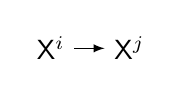
\begin{tikzpicture}[baseline=-1.5mm,-latex]
\node (C) {$\RV{X}^i$};
\node [right of = C] (A) {$\RV{X}^j$};
\draw (C) -- (A);
\end{tikzpicture} is in $\mathcal{G}$. Without loss of generality, suppose the total ordering $X^0,...,X^N$ is consistent with the partial ordering induced by $\mathcal{G}$.

Let $\kappa^i: \mathcal{E}\to \Delta(\mathcal{X}^i)$ be defined by $\kappa^i(x;A) := \mu_{|\RV{X}^<i} F_{\RV{X}^i}$. Note that by the compatibility of $\mu$, for all $x\in \mathcal{E}$, $A\in \mathcal{X}^i$ we also have
\begin{align}
    \kappa^i(x;A) = \mu_{|\PA{\mathcal{G}}{\RV{X}^i}} F_{\RV{X}^i} (x;A) \label{eq: compatibilty}
\end{align}

Consider $\kappa^{i,*}:D\times E \to \Delta(\mathcal{X}^i)$ given by \begin{align}
    \kappa^{i,*}(y,pa^i;A) := \begin{cases}\kappa^i(pa^i;A) &\RV{D}^i(y) = * \\
    \delta_{\RV{D}^i(y)}(A) & \RV{D}^i(y) \neq *\end{cases}\label{eq:passive}
\end{align}

Clearly for every $(d,pa^i) \in D\times E$ the map $A\mapsto \kappa^{i,*}(d,pa^i;A)$ is a probability distribution on $\mathcal{X}^i$. Fix $B\in\mathcal{X}_i$ and let $\kappa^{i,*}_B=\kappa'_i(\cdot;B)$.

Then for any $A\in \mathcal{B}([0,1])$
\begin{align}
    [\kappa^{i,*}_B]^{-1}(A) &= [\RV{D}^i]^{-1}(\{*\})\times[\kappa^B_i]^{-1}(A) &\text{if }0,1\not\in A\\
    &= [\RV{D}^i]^{-1}(\{*\})\times[\kappa^B_i]^{-1}(A)\cup [\RV{D}^i]^{-1}(B)\times X^{\PA{\mathcal{G}}{i}} &\text{if }1\in A\land 0\not\in A\\
    &= [\RV{D}^i]^{-1}(\{*\})\times[\kappa^B_i]^{-1}(A)\cup [\RV{D}^i]^{-1}(B^C)\times X^{\PA{\mathcal{G}}{i}} &\text{if }0\in A\land 1\not\in A\\
    &= [\RV{D}^i]^{-1}(\{*\})\times[\kappa^B_i]^{-1}(A)\cup [\RV{D}^i]^{-1}(X^i)\times X^{\PA{\mathcal{G}}{i}} &\text{if }0\in A\land 1\in A
\end{align}
Note that $\sigma(\PA{\mathcal{G}}{\RV{X}^i}\subset\mathcal{E}$ and $[\kappa^B_i]^{-1}(A)\in \sigma(\PA{\mathcal{G}}{\RV{X}^i}$. Further note that $\{*\}$, $B$ and $B^C$ are in $\sigma(\mathcal{X}^i\cup\{*\})$. Therefore, in every case the result is  an element of $\mathcal{E}\otimes\mathcal{D}$ and $\kappa^{i,*}$ is a Markov kernel.

Then $\iota^{\mathcal{G}}:D\to \Delta(\mathcal{X})$ defined below is a Markov kernel.
\begin{align}
    \iota^{\mathcal{G}}:(y;A)\mapsto \int_{A^0} \kappa^{0,*}(y;dx^0) ... \int_{A^{N-1}} \kappa^{N-1,*}(y,x^{n-2};dx^{n-1}) \kappa^{N,*}(y,x^{n-1};A^N) \label{eq:bigproduct}
\end{align}

for $y\in D$, $A\in E$ and $A^i= [\RV{X}^i]^{-1}(A)$.

From Equations \ref{eq: compatibilty}, \ref{eq:passive} and \ref{eq:bigproduct} we can verify that, given some $i\in N$, if $\RV{D}^i(y)=\{*\}$ then $[\delta_y \iota^{\mathcal{G}}]_{\PA{\mathcal{G}}{\RV{X}^i}} = \kappa_i = \mu_{\PA{\mathcal{G}}{\RV{X}^i}} F_{\RV{X}^i}$ and if $\RV{D}^i(y)\neq\{*\}$ then $\delta_y \iota^{\mathcal{G}} = \delta_{\RV{D^i}(y)} F_{\RV{X}^i}$. From Equation \ref{eq:bigproduct} and the compatibility of $\mu$ with $\mathcal{G}$ it further follows that $\delta_y\iota^\mathcal{G}$ is compatible with $\mathcal{G}$. Therefore $\delta_y \iota^\mathcal{G}=\mu^y$ and so $\iota^\mathcal{G}=\kappa^{\mu,\mathcal{G}}$.
\end{proof}

\end{document}
